\documentclass[11pt,a4paper]{article}

% --- Encoding, fonts, language ---
\usepackage[utf8]{inputenc}
\usepackage[T1]{fontenc}
\usepackage{lmodern}
\usepackage[british]{babel}
\usepackage{csquotes}

% --- Page layout & typography ---
\usepackage[margin=2.5cm]{geometry}
\usepackage{microtype}

% --- Graphics & drawing ---
\usepackage{graphicx}
\usepackage{xcolor}
\usepackage{tikz}
\usetikzlibrary{patterns, arrows.meta, calc, decorations.pathreplacing, positioning, backgrounds, fit}

% --- Math, tables, units, lists ---
\usepackage{amsmath, amssymb}
\usepackage{booktabs}
\usepackage{tabularx}
\usepackage{siunitx}
\sisetup{
  per-mode=symbol,
  range-phrase={ to },
  range-units=single,
  detect-weight=true,
  detect-family=true
}
\usepackage{enumitem}
\usepackage{caption}
\usepackage{changepage}
\usepackage{comment}
\usepackage{placeins}


% --- Bibliography ---
\usepackage{pifont}
\usepackage[backend=biber, style=apa, sortcites=true, sorting=nyt, natbib=true]{biblatex}
\addbibresource{references.bib}

% --- Hyperlinks (must be near the end; cleveref must follow hyperref) ---
\usepackage{hyperref}
\usepackage[capitalise, noabbrev]{cleveref}
\hypersetup{
  colorlinks=true,
  linkcolor=blue!60!black,
  citecolor=green!50!black,
  urlcolor=blue!70!black
}

% --- Custom commands ---
\newcommand{\TODO}[1]{\textcolor{red}{\textbf{[TODO: #1]}}}
\newcommand{\htop}{h_{\text{top}}}
\newcommand{\hbase}{h_{\text{base}}}
\newcommand{\zfloor}{z_{\text{floor}}}
\newcommand{\zceil}{z_{\text{ceil}}}
\newcommand{\pmark}{$\circ$}

\begin{document}
\begin{titlepage}
    \centering
    \vspace*{2cm}
    {\Large \textsc{Literature Research (RO57010)}}\\[0.3cm]
    {\large \textsc{Preparatory Research for Master Thesis}}\\[0.3cm]
    {\normalsize MSc Robotics, TU Delft}\\[0.2cm]
    {\small Department of Cognitive Robotics, Faculty of Mechanical Engineering}\\[2cm]

    \rule{\linewidth}{0.5mm} \\[0.4cm]
    {\LARGE \bfseries Ceiling-Aware Autonomous Navigation\\for a Reconfigurable Mobile Drilling Robot}\\[0.4cm]
    \rule{\linewidth}{0.5mm} \\[1.5cm]

    \begin{tabular}{rl}
        \textbf{Student:}           & Oscar Devos (5245982) \\[0.3em]
        \textbf{Supervisor:}        & Dr.\ Laura Ferranti (TU Delft, CoR) \\
        \textbf{Daily supervisor:}  & Riccardo Balbi (Hilti AG) \\
        \textbf{Company:}           & Hilti AG, Schaan, Liechtenstein \\
        \textbf{Period:}            & February to June 2026 \\
        \textbf{Submission:}        & 17 June 2026 \\
    \end{tabular}

    \vfill
    \begin{tabular}{c@{\hspace{2cm}}c}
        \includegraphics[height=2cm]{figures/images/tudelft_logo.png} &
        \includegraphics[height=1.8cm]{figures/images/hilti_logo.png} \\
    \end{tabular}
    \vspace{1cm}
\end{titlepage}

\newpage
\section*{Abstract}
Overhead drilling on construction sites concentrates three persistent costs: stagnant productivity at the trade level, musculoskeletal disease from arm-elevated work under tool weight and respirable crystalline silica exposure, and rework on misplaced fixings. The platform motivating this review is a wheeled, skid-steer mobile drilling robot whose effective height varies through retractable limbs and a telescoping mast, placing it outside the assumptions of classical fixed-footprint navigation. This review asks how ceiling and floor mapping with configuration-aware traversability can be implemented for real-time autonomous navigation and positioning of a reconfigurable mobile ceiling-drilling robot on embedded hardware. Six sub-questions trace the pipeline from environment representation through floor traversability, overhead clearance constraints, planning architectures, base-pose selection, and embedded deployment. Approximately 130 records, retrieved through structured arXiv and Google Scholar searches with snowball expansion and screened to peer-reviewed robotics work from 2013 onward, are surveyed taxonomically and then synthesised against the platform regime. Five gaps are consolidated: \textbf{G1}~dual-instance 2.5D floor-and-ceiling mapping on a unified-memory embedded GPU; \textbf{G2}~variance-aware overhead clearance margins, transporting chance-constraint tightening from the floor traversability literature to the second elevation layer; \textbf{G3}~joint optimisation of a planar trajectory and a continuous morphological variable carrying a dual role as transit-clearance variable and per-target task variable; \textbf{G4}~approach-aware inverse reachability that verifies a feasible configuration trajectory along the corridor rather than feasibility at the terminal pose alone; and \textbf{G5}~end-to-end characterisation of dual-instance mapping, constraint-field pipeline, and embedded receding-horizon control on a single module under concurrent perception load. No reviewed system meets all five jointly. The methodology that follows commits a dual-layer perception backbone, a variance-aware clearance field, an approach-aware goal-selection filter, and a single-stage perceptive NMPC over the augmented state $(x,y,\theta,v,\omega,s)$ on a Jetson Orin Nano Super.

\newpage
\tableofcontents
\newpage

\section{Introduction}
\label{sec:introduction}
Construction is physically demanding, slow to automate, and held back by stagnant productivity and skilled-labour shortages. Overhead drilling is among its most costly activities: years of arm-elevated work under tool weight are a leading cause of musculoskeletal disorders, drilling into reinforced concrete generates respirable crystalline silica that European and North American regulators classify as a long-term hazard, and misplaced fixings drive significant rework costs on interior finishing works. Recent advances in real-time perception and embedded optimisation now bring a robotic alternative within a cost and size range realistic for construction sites.

The platform motivating this review, described in \Cref{sec:system-description}, is a wheeled, skid-steer mobile drilling robot with a reconfigurable morphology. Its configuration-dependent collision volume and overhead workspace place it outside the assumptions of classical mobile robot navigation: the problem is inherently three-dimensional, the collision volume is itself a planning variable, and the planner must coordinate a planar trajectory with a configuration profile under hard overhead clearance constraints derived from online perception.

Each of the relevant building blocks has been studied extensively on its own: probabilistic elevation mapping, learned traversability estimation, perceptive nonlinear MPC, and inverse reachability mapping for manipulator base placement. They have not been combined for a wheeled platform of reconfigurable morphology under online-mapped overhead constraints: terrain mapping work tends not to represent ceilings, confined-space planning targets legged platforms, and goal-selection methods verify reachability at the goal pose but not along the approach trajectory. This review traces those connections, identifies the gap that emerges where they meet, and outlines a research direction in which dual-layer perception is coupled to configuration-aware planning through a constraint-field representation; the corresponding methodology is developed and evaluated in the follow-up MSc thesis. \Cref{sec:retrieval} describes how the literature was retrieved, selected, and synthesised; \crefrange{sec:sq1}{sec:sq6} review sub-questions SQ1 to SQ6 in turn; \Cref{sec:synthesis} consolidates the findings into a set of research gaps; and \Cref{sec:proposed-methodology} presents the proposed methodology that follows from them.

\subsection{Research objective}
\label{sec:research-objective}

The main research question is:


\begin{adjustwidth}{0.5em}{0.5em}
\itshape
How can ceiling and floor mapping with configuration-aware traversability be implemented for real-time autonomous navigation and positioning of a reconfigurable mobile ceiling-drilling robot on embedded hardware?
\end{adjustwidth}

\noindent Six sub-questions trace the pipeline from environment representation through to embedded deployment:

\begin{enumerate}[label=\textbf{SQ\arabic*}, leftmargin=2em, labelsep=0.5em, itemsep=0.2em, topsep=0.3em]
    \item How can floor and ceiling geometry be represented in a unified, real-time mapping framework?
    \item How is floor traversability estimated from elevation data for wheeled mobile robots?
    \item How can overhead clearance constraints be formulated for a robot with variable height?
    \item What planning and control architectures integrate floor traversability with overhead clearance?
    \item How can valid base poses for ceiling tasks be selected, including verification that the approach trajectory is feasible in the required configuration?
    \item What computational strategies enable real-time deployment of such a pipeline on embedded GPU hardware?
\end{enumerate}

\subsection{Scope}
\label{sec:scope}

The review covers ground-based wheeled mobile robots in structured indoor environments with overhead geometric constraints. Confined-space legged locomotion is included where it informs dual-layer mapping or constraint-aware control, though the target platform is wheeled. Aerial platforms and outdoor off-road traversability work are referenced only where their methods transfer to the indoor wheeled-platform setting. The review focuses on work published from approximately 2013 onward, with foundational earlier work cited where current methods build on it directly.

\section{System description}
\label{sec:system-description}

\subsection{Physical architecture}

The platform is a skid-steer wheeled robot with a rectangular base 
\begin{comment}
($\SI{0.87}{\metre} \times \SI{0.68}{\metre}$)
\end{comment}
, four retractable limbs, and a vertically telescoping drill assembly.

%
\begin{equation}
    \mathbf{q} = (\theta_1, \theta_2, \theta_3, \theta_4, \varphi_1, \varphi_2, \varphi_3, \varphi_4, q_1, q_2) \in \mathbb{R}^{10}
\end{equation}
%
where $\theta_{1\text{--}4}$ are hip joint angles controlling limb extension, 
$\varphi_{1\text{--}4}$ are wheel rotations, 
$q_1$
\begin{comment}
$\in [\SI{-0.005}{\metre}, \SI{1.280}{\metre}]$
\end{comment}
is the linear column extension, and $q_2$
\begin{comment}
$\in [\SI{0}{\metre}, \SI{0.900}{\metre}]$
\end{comment}
is the sledge adjustment.

These decouple into three operationally independent subsystems:

\begin{table}[htbp]
    \centering
    \caption{Operational subsystems.}
    \label{tab:subsystems}
    \begin{tabular}{@{}llll@{}}
        \toprule
        Subsystem & DOF & Joints & Function \\
        \midrule
        Drive       & 4 & $\varphi_{1\text{--}4}$ & Planar motion ($v_x, \omega_z$) \\
        Body pose   & 4 & $\theta_{1\text{--}4}$  & Height $h$, roll $\beta$, pitch $\alpha$ \\
        Drill reach & 2 & $q_1, q_2$              & End-effector height \\
        \bottomrule
    \end{tabular}
\end{table}

\begin{figure}[t]
  \centering
  \resizebox{0.8\linewidth}{!}{% Side-view schematic of the HILDA reconfigurable mobile drilling platform.
% Positions of LiDARs (RoboSense Airy x2) and RGBD cameras follow the
% drilly_v2 URDF: two 360-deg LiDARs on a sensor mast at z=1.16 m, providing
% simultaneous floor- and ceiling-coverage; front/rear RGBD cameras at z=0.10 m.
\begin{tikzpicture}[
    x=1cm, y=1cm,
    >={Stealth[length=2.2mm,width=1.6mm]},
    line cap=round, line join=round,
    every node/.style={font=\small},
    bodyfill/.style={fill=blue!8, draw=blue!50!black, line width=0.6pt},
    columnfill/.style={fill=gray!15, draw=black!70, line width=0.5pt},
    sledgefill/.style={fill=orange!25, draw=orange!60!black, line width=0.5pt},
    drillfill/.style={fill=red!25, draw=red!60!black, line width=0.5pt},
    wheelfill/.style={fill=gray!40, draw=black, line width=0.6pt},
    limbline/.style={draw=blue!50!black, line width=1.4pt, line cap=round},
    lidarfill/.style={fill=green!30, draw=green!40!black, line width=0.5pt},
    camfill/.style={fill=purple!25, draw=purple!50!black, line width=0.5pt},
    mastfill/.style={fill=gray!25, draw=black!60, line width=0.4pt},
    scanray/.style={draw=green!40!black, line width=0.35pt, dashed, dash pattern=on 1.4pt off 1pt},
    camray/.style={draw=purple!50!black, line width=0.35pt, dashed, dash pattern=on 1.4pt off 1pt},
    dimline/.style={<->, >={Stealth[length=1.6mm,width=1.2mm]}, draw=black!70, thin},
    helper/.style={draw=black!40, dashed, thin},
    statelabel/.style={font=\small\itshape},
  ]

  %% --- Floor --------------------------------------------------------------
  \def\floorY{0}
  \draw[line width=0.6pt] (-4.6,\floorY) -- (4.6,\floorY);
  \foreach \x in {-4.4,-4.1,...,4.5}
    \draw[draw=black!60, line width=0.3pt] (\x,\floorY) -- (\x-0.18,\floorY-0.22);
  \node[anchor=north west, font=\footnotesize] at (-4.6,\floorY-0.05) {floor};

  %% --- Wheels and limbs ---------------------------------------------------
  \def\wr{0.32}            % wheel radius (drawing units)
  \def\hipY{1.55}          % hip-plane height
  \coordinate (WL) at (-2.8,\wr);
  \coordinate (WR) at ( 2.8,\wr);
  \coordinate (HL) at (-1.6,\hipY);
  \coordinate (HR) at ( 1.6,\hipY);

  \draw[wheelfill] (WL) circle (\wr);
  \draw[wheelfill] (WR) circle (\wr);
  \fill (WL) circle (0.04); \fill (WR) circle (0.04);

  \draw[limbline] (HL) -- (WL);
  \draw[limbline] (HR) -- (WR);
  \fill[blue!50!black] (HL) circle (0.07);
  \fill[blue!50!black] (HR) circle (0.07);

  % hip-angle indicator (left limb)
  \draw[helper] (HL) -- ++(0.9,0);
  \draw[->, draw=black!70, line width=0.5pt]
    ([shift={(0.55,0)}]HL) arc[start angle=0, end angle=-50, radius=0.55];
  \node[statelabel] at ($(HL)+(0.95,-0.30)$) {$\theta$};

  %% --- Base body ----------------------------------------------------------
  \def\baseTop{2.20}
  \draw[bodyfill] (-1.85,\hipY) rectangle (1.85,\baseTop);
  \node[font=\footnotesize, text=blue!40!black] at (0,\hipY+0.32) {base};

  %% --- RGBD cameras (front +x and rear -x, mounted at base front/rear) ----
  % Front RGBD: at +x edge of base, low (URDF: 0.4, 0, 0.10)
  \def\camY{1.78}
  \draw[camfill] (1.85,\camY) rectangle ($(1.85,\camY)+(0.18,0.16)$);
  \coordinate (CF) at ($(1.85,\camY)+(0.18,0.08)$);
  \draw[camray] (CF) -- ++(0.45, 0.22) -- ++(0,-0.44) -- cycle;
  \node[font=\footnotesize, text=purple!50!black, anchor=west]
        at ($(CF)+(0.55,0.30)$) {RGBD\textsubscript{front}};

  % Rear RGBD: at -x edge of base, low (URDF: -0.4, 0, 0.10)
  \draw[camfill] ($(-1.85,\camY)+(-0.18,0)$) rectangle (-1.85,\camY+0.16);
  \coordinate (CR) at ($(-1.85,\camY)+(-0.18,0.08)$);
  \draw[camray] (CR) -- ++(-0.45, 0.22) -- ++(0,-0.44) -- cycle;
  \node[font=\footnotesize, text=purple!50!black, anchor=east]
        at ($(CR)+(-0.55,0.30)$) {RGBD\textsubscript{rear}};

  %% --- Drill column (retracted) ------------------------------------------
  \def\colTop{4.05}
  \draw[columnfill] (-0.35,\baseTop) rectangle (0.35,\colTop);
  \node[font=\footnotesize, rotate=90, text=black!60]
        at (-0.55,(\baseTop+\colTop)/2) {column};

  %% --- Sensor mast + two Airy LiDARs (z=1.16 m in URDF) ------------------
  % A short post lifts a horizontal profile that carries two LiDARs back-to-back.
  % We draw the mast offset in +x so it does not collide with the drill column.
  \def\mastX{0.85}                 % mast x-position
  \def\profileY{2.95}              % top of mast / base of horizontal profile
  \def\lidY{3.10}                  % LiDAR centre height
  % vertical post
  \draw[mastfill] (\mastX-0.06,\baseTop) rectangle (\mastX+0.06,\profileY);
  % horizontal sensor profile (heat-sink) carrying the two LiDARs
  \draw[mastfill] (\mastX-0.30,\profileY) rectangle (\mastX+0.30,\profileY+0.08);
  % rear LiDAR (on the -x end of the profile, faces rearward)
  \coordinate (LR) at (\mastX-0.22,\lidY);
  \draw[lidarfill] ($(LR)+(-0.08,-0.08)$) rectangle ($(LR)+(0.08,0.08)$);
  % front LiDAR (on the +x end of the profile, faces forward)
  \coordinate (LF) at (\mastX+0.22,\lidY);
  \draw[lidarfill] ($(LF)+(-0.08,-0.08)$) rectangle ($(LF)+(0.08,0.08)$);
  \coordinate (LCTR) at (\mastX,\lidY);

  % Combined coverage: one slim cone up to ceiling. Down-coverage is implied
  % by the label (drawing it would pierce the base body in a side view).
  \draw[scanray] (LCTR) -- ($(LCTR)+(-0.55, 2.95)$);
  \draw[scanray] (LCTR) -- ($(LCTR)+( 0.00, 3.10)$);
  \draw[scanray] (LCTR) -- ($(LCTR)+( 0.55, 2.95)$);

  % LiDAR label with leader line, placed in the clear region to the right.
  \node[font=\footnotesize, text=green!30!black, anchor=west]
        (LIDARLBL) at (1.85,\lidY+0.55) {2$\times$ Airy LiDAR};
  \node[font=\scriptsize, text=green!30!black, anchor=west]
        at (1.85,\lidY+0.28) {(floor $+$ ceiling)};
  \draw[draw=green!40!black, line width=0.35pt]
        ($(LF)+(0.10,0.04)$) -- (1.83,\lidY+0.55);

  %% --- Sledge (q1 extension) ---------------------------------------------
  \def\sledgeTop{5.10}
  \draw[sledgefill] (-0.28,\colTop) rectangle (0.28,\sledgeTop);

  %% --- Drill assembly (q2 sledge adjustment) -----------------------------
  \def\drillTop{5.85}
  \draw[drillfill] (-0.22,\sledgeTop) rectangle (0.22,\drillTop);
  \draw[fill=black!75, draw=black] (-0.05,\drillTop) rectangle (0.05,\drillTop+0.25);
  \coordinate (DT) at (0,\drillTop+0.25);

  %% --- Ceiling ------------------------------------------------------------
  \def\ceilY{6.55}
  \draw[line width=0.6pt] (-4.6,\ceilY) -- (4.6,\ceilY);
  \foreach \x in {-4.4,-4.1,...,4.5}
    \draw[draw=black!60, line width=0.3pt] (\x,\ceilY) -- (\x+0.18,\ceilY+0.22);
  \node[anchor=south west, font=\footnotesize] at (-4.6,\ceilY+0.05) {ceiling};

  %% --- Dimension lines (right side: vertical state stack) ----------------
  \def\dimX{3.55}
  % short helpers only — long horizontal dashes across the figure are clutter
  \draw[helper] (1.85,\hipY) -- (\dimX+0.15,\hipY);
  \draw[dimline] (\dimX,\floorY) -- (\dimX,\hipY)
        node[midway, right=1pt, statelabel] {$\hbase$};

  \draw[helper] (0.35,\colTop) -- (\dimX+0.15,\colTop);
  \draw[dimline] (\dimX,\hipY) -- (\dimX,\colTop)
        node[midway, right=1pt, statelabel] {$h_{\text{col}}$};

  \draw[helper] (0.28,\sledgeTop) -- (\dimX+0.15,\sledgeTop);
  \draw[dimline] (\dimX,\colTop) -- (\dimX,\sledgeTop)
        node[midway, right=1pt, statelabel] {$q_1$};

  \draw[helper] (0.22,\drillTop) -- (\dimX+0.15,\drillTop);
  \draw[dimline] (\dimX,\sledgeTop) -- (\dimX,\drillTop)
        node[midway, right=1pt, statelabel] {$q_2$};

  % h_top (floor to drill tip)
  \def\dimXf{4.45}
  \draw[helper] (DT) -- (\dimXf+0.15,\drillTop+0.25);
  \draw[dimline] (\dimXf,\floorY) -- (\dimXf,\drillTop+0.25)
        node[midway, right=1pt, statelabel] {$\htop$};

  %% --- Wheel radius and limb length (left side) --------------------------
  \def\dimL{-3.55}
  \draw[helper] (WL) ++(-\wr,0) -- (\dimL-0.15,\wr);
  \draw[dimline] (\dimL,\floorY) -- (\dimL,\wr)
        node[midway, left=1pt, statelabel] {$r$};
  \node[statelabel, rotate=53, anchor=south]
        at ($(WL)!0.5!(HL)+(-0.12,0.05)$) {$\ell$};

  %% --- World frame (bottom-left corner) ----------------------------------
  \begin{scope}[shift={(-4.2,0.25)}]
    \draw[->, line width=0.6pt] (0,0) -- (0.7,0) node[right=-1pt, font=\footnotesize] {$x$};
    \draw[->, line width=0.6pt] (0,0) -- (0,0.7) node[above=-1pt, font=\footnotesize] {$z$};
  \end{scope}

  %% --- Forward velocity and yaw-rate hints -------------------------------
  % placed above the base body, clear of the RGBD cameras
  \draw[->, line width=0.6pt, draw=blue!50!black]
        (1.30,\baseTop+0.30) -- ++(0.55,0)
        node[right=-1pt, font=\footnotesize, text=blue!40!black] {$v_x$};
  \draw[->, line width=0.6pt, draw=blue!50!black]
        (-1.20,\baseTop+0.25) arc[start angle=-20, end angle=210, radius=0.18];
  \node[font=\footnotesize, text=blue!40!black, anchor=east]
        at (-1.45,\baseTop+0.30) {$\omega_z$};

\end{tikzpicture}
}
  \caption{Platform configuration with state variables and onboard sensors.}
  \label{fig:platform}
\end{figure}

\subsection{Height profile}

The robot's total height above the floor contact point is:
%
\begin{equation}
    \htop = \underbrace{\hbase}_{\text{limbs}} + \underbrace{h_{\text{col}}}_{\text{column base}} + \underbrace{q_1 + q_2}_{s} \; [\si{\metre}]
    \label{eq:htop}
\end{equation}
%
where $h_{\text{col}}$ is the fixed column-base offset (from the hip plane to the top of the retracted column), $s = q_1 + q_2$ is the combined sledge extension, and $\hbase = l\sin\theta + r - h_0$ is the base height, with $l$, $r$, and $h_0$ denoting fixed limb-geometry parameters (limb-segment length, wheel radius, and hip-frame vertical offset, respectively). The limb controller enforces symmetric hip angles ($\theta_1 = \theta_3$, $\theta_2 = \theta_4$), so a single representative angle~$\theta$ suffices on flat ground. Stability is guaranteed only within a bounded floor slope.

\begin{comment}
% h_col     = 1.899 m   (URDF-derived, hip plane to top of retracted column)
% l         = 0.15  m
% r         = 0.104 m
% h_0       = 0.021 m
% max slope = 5 deg
\end{comment}

Total height ranges from \SI{1.98}{\metre} (fully retracted) to \SI{4.17}{\metre} (fully extended). This variation makes ceiling clearance a configuration-dependent planning problem rather than a fixed safety margin.

\subsection{Sensing and compute}
Two sensor modalities feed a dual-computer architecture. State estimation (SLAM-based localisation and odometry) runs on an existing UDOO pipeline and is assumed accurate; improving localisation is out of scope.

\paragraph{Sensors.}
\begin{itemize}[nosep]
    \item \textbf{Dual Robosense Airy 96 LiDARs}, sledge-mounted, give
    \ang{360} coverage of floor and ceiling and serve as the primary input to the existing elevation mapping pipeline, as well as for obstacle detection during transit.
    \item \textbf{Three Intel RealSense D455 depth cameras}, also sledge-mounted. Two sit beneath the LiDARs, providing forward and backward facing RGBD that complement the LiDARs for close-range and dynamic obstacle detection in transit. The third faces upward beside the drill and is active during approach and drilling, supporting (1)~ceiling-object classification (drillable vs.\ obstructed) and (2)~visual servoing for sub-centimetre drill alignment.
\end{itemize}

\paragraph{Compute.}
A UDOO Bolt V8 (Ubuntu 24.04, ROS\,2 Jazzy) handles low-level motor control, state estimation, and networking. An NVIDIA Jetson Orin Nano Super runs the perception--planning pipeline central to this thesis: environment perception, traversability estimation, constraint field computation, and motion planning. JetPack 6.2 ships with Ubuntu 22.04 (ROS\,2 Humble), so the Jetson runs a ROS\,2 Jazzy Docker container, matching the UDOO's distribution and removing the need for cross-version DDS bridging.

\subsection{Operational workflow}
\label{sec:operational-workflow}
The platform targets mid-size indoor construction sites with ceilings up to \SI{4}{\metre}. A drilling mission proceeds as: (1)~receive ceiling drill targets from a BIM-based operator plan; (2)~plan a path considering floor traversability, ceiling clearance, and dynamic obstacles; (3)~navigate while adjusting body height to maintain clearance; (4)~position at the target base pose; (5)~extend the sledge, classify the ceiling surface with the upward-facing camera, and if drillable, execute the drilling operation. Steps~2--4 are the perception--planning problem this study addresses; step~5 falls to the ceiling classification module described in \Cref{sec:meth:goals}.

Three bounds scope the methods examined in later chapters. The local map must cover \SIrange{7}{10}{\metre} around the platform at \SIrange{5}{10}{\centi\metre} cell resolution and update at $\geq\SI{5}{\hertz}$. End-to-end perception-to-control latency must stay below \SI{50}{\milli\second} to support a \SI{20}{\hertz} control rate. The full pipeline must run on the embedded compute introduced above.

\section{Literature retrieval methodology}
\label{sec:retrieval}

The primary database was arXiv, covering January~2013 to April~2026, with parallel searches on Google~Scholar using the same Boolean strings (\Cref{tab:retrieval}). Results were screened by title; abstracts of candidates were then read and the record assigned to the relevant sub-question collection in Zotero. From the most relevant papers in each collection, the reference lists were followed to pull in further sources from IEEE~Xplore, Scopus, Web~of~Science, Springer, and other publishers. The time window opens with the volumetric and multi-level surface representations against which modern dual-layer designs are still compared \citep{OctoMapEfficientProbabilistic, MultiLevelSurfaceMaps}; earlier foundational works were retained where current methods build on them directly. Only English sources were considered.

As an additional source of candidates, Claude AI's deep research mode was run once per sub-question. Every returned item was manually retrieved, read against the inclusion criteria below, and verified against the underlying publication; only those that passed were added to Zotero.

\begin{table}[h]
\centering
\footnotesize
\caption{Boolean search strings per sub-question. \texttt{*} denotes a
wildcard.}
\label{tab:retrieval}
\begin{tabular}{@{}p{0.04\linewidth}p{0.90\linewidth}@{}}
\toprule
SQ & Search string \\
\midrule
SQ1 & (\texttt{"elevation map*"} OR \texttt{"multi-level surface"} OR
       \texttt{"dual-layer map"} OR \texttt{"point cloud tomography"}) AND
       (\texttt{"mobile robot"} OR \texttt{legged} OR \texttt{wheeled}) AND
       (\texttt{ceiling} OR \texttt{overhead} OR \texttt{"confined space"}) \\
SQ2 & (\texttt{traversability} OR \texttt{"terrain classification"}) AND
       (\texttt{elevation} OR \texttt{"height map"} OR \texttt{"point cloud"})
       AND (\texttt{geometric*} OR \texttt{learn*} OR \texttt{self-supervis*}
       OR \texttt{"reinforcement learning"}) \\
SQ3 & (\texttt{"ceiling clearance"} OR \texttt{"overhead constraint*"} OR
       \texttt{"variable height"} OR \texttt{reconfigurable}) AND
       (\texttt{"collision check*"} OR \texttt{"signed distance"} OR
       \texttt{"safety margin"}) \\
SQ4 & (\texttt{NMPC} OR \texttt{"model predictive"} OR \texttt{MPPI} OR
       \texttt{"control barrier"} OR \texttt{"state lattice"}) AND
       (\texttt{perceptive} OR \texttt{elevation} OR \texttt{clearance}) AND
       (\texttt{wheeled} OR \texttt{quadruped} OR \texttt{mobile}) \\
SQ5 & (\texttt{"inverse reachability"} OR \texttt{"capability map"} OR
       \texttt{"base placement"} OR \texttt{"task sequencing"}) AND
       (\texttt{"mobile manipulator"} OR \texttt{overhead} OR \texttt{BIM}) \\
SQ6 & (\texttt{Jetson} OR \texttt{"embedded GPU"} OR \texttt{"real-time"}) AND
       (\texttt{acados} OR \texttt{TensorRT} OR \texttt{CuPy} OR
       \texttt{nvblox} OR \texttt{NMPC} OR \texttt{"elevation mapping"}) \\
\bottomrule
\end{tabular}
\end{table}

A record was included if it (i)~addressed at least one sub-question on a wheeled or legged ground platform, an aerial platform with methodological transfer to ground navigation, or a mobile manipulator; (ii)~contributed algorithm, system integration, or experiment; and (iii)~appeared in a peer-reviewed robotics venue or as an arXiv preprint. Pure semantic segmentation without a geometric or planning component, planetary-rover work whose terrain assumptions do not transfer to indoor construction sites, outdated surveys, and short workshop abstracts were excluded.

After deduplication and screening, approximately 130 records were retained, organised per sub-question in Zotero.

\section{SQ1: Environment representation}
\label{sec:sq1}

A robot navigating under overhead constraints must maintain a spatial model of both the surface it drives on and the structures above it. This section reviews the representations available for this purpose, organised by their dimensionality and structural assumptions.

\begin{figure}[t]
  \centering
  \includegraphics[width=\linewidth]{figures/images/SQ1_visu.png}
  \caption{TODO}
  \label{fig:irm}
\end{figure}

\subsection{2.5D elevation mapping}
\label{sec:sq1:elevation}

The dominant representation for terrain-aware mobile robot navigation is the 2.5D elevation map: a regular $(x,y)$ grid where each cell stores a single height value. \citet{fankhauserROBOTCENTRICELEVATIONMAPPING2014} introduced robot-centric elevation mapping with Kalman-filter fusion of range measurements and explicit handling of pose drift, targeting legged robots whose state estimate cannot be assumed globally consistent. \citet{UniversalGridMap2025} subsequently published the \texttt{grid\_map} library, which provides the C++ data structure and ROS interface underlying most subsequent elevation mapping work. \citet{fankhauserProbabilisticTerrainMapping2018} extended the formulation by propagating the full six-dimensional pose covariance into the per-cell height estimate, yielding a probabilistic map with explicit upper and lower confidence bounds. Crucially, the method requires no absolute localisation: it operates on proprioceptive estimates alone, which makes it robust in the long-duration, sensor-degraded conditions typical of construction environments.

\citet{mikiElevationMappingLocomotion2022} ported the pipeline to GPU in \texttt{elevation\_mapping\_cupy}, achieving real-time map updates on Jetson hardware and exposing post-processing as CuPy plugins, including learned traversability filters, ray-cast cleanup, and plane segmentation. This is the mapping framework adopted as the perception backbone of the present work. \citet{erniMEMMultiModalElevation2023} extended the GPU framework to fuse appearance and semantic information from cameras alongside geometric LiDAR returns, producing multi-modal layers that downstream components can consume in a uniform way.

\citet{GEMOnlineGlobally} take a different design point. The same local robot-centric grid is kept for fast updates, but a global layer of submaps sits underneath it, re-posed rather than rebuilt when SLAM closes a loop. The \texttt{elevation\_mapping\_cupy} window stays strictly local and pays nothing for global consistency; GEM accepts a latency cost to preserve it across revisits.

A recurring failure mode of robot-centric 2.5D maps is missing data from self-occlusion and limited field-of-view. Learned completion methods address it within the same paradigm: \citet{stolzleReconstructingOccludedElevation2021} train a self-supervised U-Net against synthetic ray-cast occlusion, and \citet{yangRealtimeNeuralDense2023} reconstruct a dense grid from sparse LiDAR with per-pixel uncertainty. Both operate as plug-ins to a 2.5D map rather than replacements for it; the uncertainty layer of the latter is the input to the variance-aware constraint tightening reviewed in
\Cref{sec:sq3}.

\citet{grandiaPerceptiveLocomotionNonlinear2022} precompute steppability classification, plane segmentation, and a signed distance field per elevation map, then embed convex inequalities derived from these structures inside a real-time NMPC. 2.5D data is therefore consumable as a constraint source for gradient-based receding-horizon control, regardless of the specific architecture chosen in \Cref{sec:sq4}.

A 2.5D grid stores one height per cell; either the floor below or the ceiling above, not both. For a robot whose feasibility depends on the corridor between the two surfaces, this is insufficient.

\subsection{3D volumetric representations}
\label{sec:sq1:volumetric}

Full 3D representations avoid the single-surface limitation of 2.5D elevation maps by modelling occupied space as a volume. Probabilistic octrees \citep{OctoMapEfficientProbabilistic}, hashed TSDF and ESDF blocks \citep{millaneNvbloxGPUAcceleratedIncremental2024}, and surfel grids \citep{droeschelContinuousMappingLocalization2017} are the dominant design points. All three encode distance to the nearest occupied surface without distinguishing whether that surface lies above or below the body, so a configuration-dependent clearance field has to be reconstructed from the underlying geometry rather than read off the map; nvblox's continuous ESDF provides analytic gradients that a gradient-based planner can consume directly, but it still does not distinguish floor from ceiling. At the cell sizes required for navigation, their memory footprint also exceeds what the target embedded platform can hold.

Two volumetric systems sit closer to overhead-constrained ground navigation but neither serves as a primary backbone. \citet{freyLocomotionPolicyGuided2022} argued explicitly against 2.5D for confined-space locomotion, on the grounds that elevation maps lose information about overhangs and narrow gaps that voxels preserve, and trained a sparse 3D convolutional network to regress traversability from a robot-centric voxel-occupancy grid under massively parallel locomotion simulation. The output is an end-to-end learned cost rather than an explicit clearance constraint, which precludes hard-constraint formulations on the optimiser side, and the supervision is conditioned on a quadrupedal policy whose body height is continuously controllable; transfer to a wheeled chassis with discrete reconfiguration through retractable limbs and a telescoping mast has not been demonstrated. \citet{garroteHMAPsHybridHeight2018} combine a 2.5D grid for the dominant ground surface with local voxel patches where geometric complexity demands them, preserving overhangs locally at memory cost comparable to an elevation map; the implementation is CPU-only and produces a discrete patch-based output that does not yield a smooth clearance field.

A more recent paradigm replaces implicit volumetric grids with explicit anisotropic primitives. \citet{kerbl20233dgs} introduced 3D Gaussian Splatting, representing a scene as a cloud of oriented Gaussians rasterisable above \SI{100}{\hertz} at 1080\,p with optimisation orders of magnitude faster than neural radiance fields; robotic adaptations followed quickly on aerial platforms \citep{chenSplatNavSafeRealTime2025} and wheeled ground vehicles \citep{taoRTGuIDERealTimeGaussian2025}. For complex ceiling geometry such as HVAC ducts, cable trays, and structural beams, 3DGS captures fine overhead detail more faithfully than any 2.5D surface representation. Three properties limit adoption as a primary representation: the Gaussian cloud does not natively decompose into floor and ceiling surfaces; existing rasterisers target image-space rendering rather than the analytic field queries a gradient-based planner consumes; and the published systems are camera-driven and untested within the latency and memory budget of an embedded GPU comparable to the target platform. 3DGS is therefore retained as a candidate for future work where photorealistic ceiling reconstruction is the primary requirement, not adopted here.

A field-scale perspective on these volumetric primitives comes from the integrated stacks deployed in confined subterranean autonomy~\citep{azpuruaSurveyAutonomousExploration2023}, where ceiling clearance is treated, where it is treated at all, as an attribute of the volumetric occupancy field rather than a planning quantity. The two landmark DARPA Subterranean Challenge winners, Team CoSTAR's NeBula~\citep{aghaNeBulaQuestRobotic2021} and Team CERBERUS~\citep{tranzattoTeamCERBERUSWins2024}, both ran on volumetric occupancy with overhead geometry included implicitly through 3D collision checking against an inflated robot body. This is sufficient for cave, tunnel, and urban exploration under permissive vertical clearance, but not for a platform whose effective height is itself a planning variable. The closest wheeled hardware analogue, the skid-steer underground-mining platform of \citet{tatschRhinoAutonomousRobot2023}, reduces ceiling geometry to a binary obstacle classification by a fixed height threshold even on a platform that already captures the relevant ceiling data online.

\subsection{Multi-level surface maps}
\label{sec:sq1:mls}

Multi-level surface (MLS) maps~\cite{MultiLevelSurfaceMaps} extend 2.5D elevation maps by allowing \emph{multiple} surface patches per $(x,y)$ cell, each with an elevation, variance, and surface type. This captures overhangs, tunnels, and multi-storey structures within a grid framework without the memory cost of full volumetric discretisation.

\citet{lodhiTraversability_generator3dLibrary3D2026} recently released \texttt{traversability\_generator3d}, a C++ library that converts an MLS map into a \texttt{TraversabilityMap3d} through RANSAC plane fitting on each surface patch and footprint-aware geometric analysis (slope, step height, body collision against the fitted patches). \citet{bockmannUgv_nav4dAdvancedMultiSurface2024} embed this in \texttt{ugv\_nav4d}, an SBPL-based ARA$^*$ planner over motion primitives in the four-dimensional state $(x,y,z,\theta)$, with an accompanying \texttt{ugv\_nav4d\_ros2} wrapper that consumes streaming pointcloud topics from an online SLAM front end. This is the most complete multi-surface navigation pipeline for wheeled ground vehicles currently available in open source.

Two limitations qualify the real-time claim. First, the \texttt{ugv\_nav4d} documentation states that the \texttt{TraversabilityMap3d} has to be fully expanded from the MLS before planning starts, and that on-the-fly expansion during planning is untested and a likely source of bugs when parallelism is enabled. The map is therefore rebuilt once per planning cycle rather than updated continuously as the robot moves, and the pipeline is best matched to a periodic global planner rather than to a closed-loop controller. Second, the output of the traversability stage is a graph of discrete node classes, well matched to the search-based planner above it but not a smooth continuous field.

The second property is the more consequential for the planning architectures admitted by \Cref{sec:sq4}. Gradient-based receding-horizon controllers, one of the families considered there, consume constraint fields that are at least $C^1$-smooth, with bounded gradients computable at every queried point along the prediction horizon. RANSAC plane fitting and per-patch classification produce discontinuous outputs at patch boundaries that violate this requirement. The MLS pipeline therefore does not serve as a primary backbone for that family of controllers, independent of its real-time properties.

\citet{yangEfficientGlobalNavigational2024} address the multi-surface problem through Point Cloud Tomography (PCT), which slices a global pointcloud into a stack of equidistant horizontal tomograms, each consisting of a paired ground elevation, ceiling elevation, and travel-cost layer on a shared 2.5D grid. Traversability is computed from terrain gradient on the ground layer combined with an interval cost $c_I = \alpha_d(d_{\text{ref}} - d_I)$ that penalises ground-to-ceiling gaps below a configurable preferred height $d_{\text{ref}}$, with intervals below an absolute minimum $d_{\min}$ forbidden outright. A modified A$^*$ search then traverses the slice stack through gateway cells: planar positions where an adjacent slice carries lower cost above or below. The resulting trajectory is post-processed by a polynomial optimisation that adjusts the body height $q_z(t)$ between $H_g(q(t))$ and $H_c(q(t))$. PCT evaluates scenes roughly three orders of magnitude faster than dense voxel baselines, with several-millisecond evaluation in real-world experiments on a quadrupedal platform with onboard NVIDIA Jetson AGX Orin compute.

PCT is the published system most structurally similar to the navigation problem treated in this review: it represents both floor and ceiling on a shared 2.5D grid, encodes clearance as an explicit cost, and admits configuration-dependent planning through body-height adjustment. Three properties prevent its direct adoption as the perception backbone here. The tomogram is constructed from a pre-built global pointcloud produced by an offline SLAM run with manual removal of dynamic points and noise; no robot-centric construction during motion is demonstrated. The platform shown is a quadruped, whose body height is treated as a continuous variable in the trajectory optimisation, whereas the wheeled, reconfigurable platform considered in this work changes effective height through the discrete actuation of retractable limbs and a telescoping column. The per-cell cost layers and the gateway transitions between slices are also discrete by construction, so PCT inherits the same gradient-continuity limitation as the MLS pipeline above.

\subsection{Dual and multi-layer elevation maps}
\label{sec:sq1:dual}

\citet{buchananWalkingPostureAdaptation2019} introduce a robot-centric \emph{multi-elevation map} within the Fankhauser/\texttt{grid\_map} lineage, maintaining separate floor and ceiling layers. Incoming range measurements are partitioned into floor and ceiling sets via a Bayesian MAP estimate that uses a body-height-conditioned elevation prior, after which each layer is fused independently with the standard one-dimensional Kalman update at the cell level. A signed distance field is computed from the dual map and queried by a CHOMP-based trajectory optimiser, with the robot represented as a \emph{deformable bounding box} whose vertical extent is coupled to the planned posture. The system is demonstrated on the hexapod Weaver under \SI{25}{\centi\metre} overhangs and through \SI{70}{\centi\metre} gaps, in artificial test arenas and realistic environments.

\citet{PerceptiveWholebodyPlanning} extend the same formulation to a quadrupedal platform of substantially greater scale. ANYmal, with a nominal standing height of \SI{80}{\centi\metre} and a width of \SI{59}{\centi\metre}, navigates through openings as small as \SI{60}{\centi\metre} using onboard mapping without prior knowledge of the environment. The planner is hierarchical: an RRT-Connect search produces an initial body-pose trajectory in roughly \SI{100}{\milli\second} on dedicated onboard compute, the trajectory is then smoothed by CHOMP against the SDF of the dual map, and footholds are updated from terrain scores derived from the floor layer. End-to-end re-planning over three-metre trajectories runs at a \SI{500}{\milli\second} cycle, with field validation at an emergency rescue training facility. The system is the most extensively validated dual-layer mapping pipeline coupled to a perceptive whole-body planner currently published.

\citet{mikiLearningWalkConfined2024}, from the same group, take a different route. The two coupled 2.5D layers are replaced by a 3D voxel occupancy grid (\(32 \times 32 \times 32\) at \SI{0.08}{\metre} resolution), and the explicit SDF and trajectory optimiser are replaced by a two-layer hierarchical reinforcement-learning policy. A high-level network reads the voxel grid and emits a six-dimensional command (linear and angular velocity, roll, pitch, body height) to a low-level perceptive locomotion controller; a procedural terrain generator based on Wave Function Collapse supplies diverse training environments with overhanging and rough-terrain features. The system shows more agile confined-space behaviour than the Buchanan pipelines. Two properties of the dual-layer formulation are no longer exposed: there is no explicit clearance field that an optimisation-based planner can consume as a constraint, and posture adaptation is mediated by a learned policy on a quadruped whose body height is a continuous, gait-mediated degree of freedom rather than the output of a discrete mechanical reconfiguration.

The dual-layer lineage establishes the feasibility of two coupled 2.5D layers fused within the GridMap framework, supporting real-time floor-and-ceiling mapping with onboard compute and yielding a signed distance field consumable by gradient-based trajectory optimisation. Two elements remain absent in this body of work. The platform regime is legged in every published instance (hexapod, quadruped, RL-controlled quadruped), and a wheeled chassis whose effective height varies through discrete reconfiguration of retractable limbs and a telescoping mast is therefore unaddressed. The downstream interface is also tied to a sampling-and-smoothing planner with a deformable-body collision primitive, rather than to a query interface that closed-loop optimisation-based planners admit directly. Buchanan's static safety margins predate the variance-aware tightening principle taken up in \Cref{sec:sq3:uncertainty}, which exploits the per-cell variance the dual-layer formulation already produces. The perception design developed in \Cref{sec:proposed-methodology} returns to these elements.

\subsection{BIM-prior maps}
\label{sec:sq1:bim}

In construction environments, a Building Information Model (BIM) carries geometric and semantic information about the structure being built: ceiling heights, beam locations, duct routing, and structural columns. BIM is therefore a candidate spatial representation that downstream planners could consume in place of, or alongside, an online perception stack.

The canonical BIM-to-ROS pipeline is that of \citet{kimDevelopmentBIMintegratedConstruction2021}, who developed an Industry Foundation Classes to Simulation Description Format converter that exposes BIM geometry to ROS-based simulation, navigation, and motion planning, demonstrated on an indoor wall-painting case study. The closest deployed industrial precedent, the Hilti Jaibot \citep{hilti2020jaibot}, uses BIM as the source of drill target coordinates and an approximate ceiling reference; navigation is teleoperated, metric localisation comes from a robotic total station, and only the drilling pattern within reach is executed autonomously against the model. A second-generation update added on-board sensing of corrugated metal-deck profiles to adapt planned holes to as-built deviations, evidence that the BIM alone is not a sufficient representation. \citet{blum2020}, working with the same industrial partner, report typical as-built deviations of several centimetres on a real construction site, large enough that global registration against the BIM mesh fails without local re-referencing; on platforms whose vertical clearance budget is itself of order centimetres, that magnitude of error makes a BIM-derived clearance unreliable as a hard constraint. The BIM also does not encode temporary structures or dynamic actors: scaffolding, formwork, packaging, and human workers all appear in the sensor stream without ever being represented in the model.

BIM data therefore retains value as a source of high-level priors and task targets, including candidate drill positions, structural element classification, and initial estimates of ceiling height, but it cannot replace real-time sensing for safe overhead-constrained navigation. The appropriate consumer of BIM in such a system is the goal-selection layer (\Cref{sec:sq5}), not the perception layer.

\subsection{Summary: representation gap for embedded dual-layer mapping}
\label{sec:sq1:discussion}

\Cref{tab:sq1_comparison} consolidates the reviewed representations against four requirements implicit in the platform and task: dual floor-and-ceiling geometry, robot-centric construction during motion, real-time updates within the memory and compute envelope of an embedded GPU, and a query interface compatible with the planning architectures of \Cref{sec:sq4}. No reviewed system clears all four at once. The dual-layer lineage of \citet{buchananWalkingPostureAdaptation2019,PerceptiveWholebodyPlanning} and the multi-surface pipelines of \citet{lodhiTraversability_generator3dLibrary3D2026,bockmannUgv_nav4dAdvancedMultiSurface2024,yangEfficientGlobalNavigational2024} are the closest published matches but each meets a strict subset: the dual-layer line is legged-only with a deformable-body sampler downstream, and the MLS and PCT pipelines are built from offline-fused global point clouds with discrete per-cell classifications that the candidate gradient-based controllers of \Cref{sec:sq4} cannot consume directly. The successor learned policy of \citet{mikiLearningWalkConfined2024} achieves more agile confined-space behaviour but removes the explicit clearance representation any optimisation-based downstream planner requires, and BIM as a primary representation~\citep{kimDevelopmentBIMintegratedConstruction2021,hilti2020jaibot,blum2020} fails on as-built deviation magnitudes relative to ceiling-clearance margins. The backbone that simultaneously meets all four requirements is described in \Cref{sec:proposed-methodology}.

\begin{table}[htbp]
    \centering
    \captionsetup{font=small}
    \caption{Comparison of environment representations for overhead-constrained navigation. Columns four and five record the two query interfaces required by the candidate planning architectures considered in~\Cref{sec:sq4}; \checkmark indicates the representation natively supplies the interface, \emph{partial} indicates it is reachable only through additional non-trivial processing.}
    \label{tab:sq1_comparison}
    \resizebox{\textwidth}{!}{%
    \begin{tabular}{@{}lccccc@{}}
        \toprule
         & Floor + & Real-time & Embedded & Continuous & Plane \\
         & ceiling & robot-centric & GPU & diff.\ field\textsuperscript{$\dagger$} & decomp.\textsuperscript{$\ddagger$} \\
        \midrule
        Elevation map~\cite{mikiElevationMappingLocomotion2022}                     & ---        & \checkmark & \checkmark & \checkmark & partial    \\
        OctoMap~\cite{OctoMapEfficientProbabilistic}                                 & implicit   & \checkmark & ---        & ---        & ---        \\
        nvblox~\cite{millaneNvbloxGPUAcceleratedIncremental2024}                     & implicit   & \checkmark & \checkmark & partial    & partial    \\
        Surfel grid~\cite{droeschelContinuousMappingLocalization2017}                & implicit   & \checkmark & ---        & ---        & ---        \\
        3DGS~\cite{chenSplatNavSafeRealTime2025,taoRTGuIDERealTimeGaussian2025}       & implicit   & partial    & partial    & ---        & partial    \\
        MLS + trav3d~\cite{lodhiTraversability_generator3dLibrary3D2026,bockmannUgv_nav4dAdvancedMultiSurface2024} & \checkmark & partial    & ---        & ---        & partial    \\
        PCT~\cite{yangEfficientGlobalNavigational2024}                               & \checkmark & ---        & \checkmark & ---        & ---        \\
        Buchanan~\cite{buchananWalkingPostureAdaptation2019,PerceptiveWholebodyPlanning} & \checkmark & \checkmark & ---        & \checkmark & ---        \\
        BIM prior~\cite{kimDevelopmentBIMintegratedConstruction2021}                 & \checkmark & ---        & n/a        & \checkmark & \checkmark \\
        \textbf{Proposed (this work)}                                                & \checkmark & \checkmark & \checkmark & \checkmark & \checkmark \\
        \bottomrule
    \end{tabular}%
    }
    \smallskip
    {\footnotesize
    \par\noindent\textsuperscript{$\dagger$}\,Continuous differentiable field: provides $C^1$-smooth, gradient-queryable scalar values directly consumable as inequality constraints or costs in gradient-based online trajectory optimisation.
    \par\noindent\textsuperscript{$\ddagger$}\,Plane decomposition: provides explicit piecewise-affine surface primitives directly consumable as polytopic constraints in receding-horizon tightening hierarchies.
    }
\end{table}

\FloatBarrier

\section{SQ2: Traversability estimation from elevation and terrain data}
\label{sec:sq2}

A wheeled platform navigating an indoor construction site must convert the geometry of the floor it observes into a scalar cost the planner can consume. This section reviews the methods that produce such a cost from elevation data, organised by their progression from hand-crafted geometric features, through supervised learning on elevation grids, to self-supervised and reinforcement-learning approaches.

\subsection{Geometric filter pipelines}
\label{sec:sq2:geometric}

The classical approach derives traversability from local surface descriptors computed over a sliding window of the elevation map. Three features dominate: \emph{slope} (the inclination of a plane fitted to a local neighbourhood), \emph{roughness} (the residual variance of the elevation samples after plane fitting), and \emph{step height} (the maximum elevation discontinuity within the kernel). \citet{chilian2009} introduced the weighted sum of all three, normalised against critical thresholds, as a single danger value on stereo-derived elevation grids; the template has anchored non-trainable traversability ever since. \citet{wermelingerNavigationPlanningLegged2016} adapted it to the probabilistic robot-centric elevation map of \Cref{sec:sq1} and introduced \emph{footprint traversability}: the per-cell scores are convolved over the robot's footprint polygon, so that a pose centred next to a step is penalised even when the centre cell itself is smooth. The same paper packages the filters as a composable chain in the \texttt{grid\_map\_filters} package, parametrised by per-feature weights and critical values, which has since become the de facto reference implementation for elevation-grid traversability in the ROS ecosystem.

The pipeline ports to embedded compute without algorithmic compromise. \citet{mikiElevationMappingLocomotion2022} reimplement the geometric filters as CuPy kernels that run inside the elevation map update cycle, with reported per-update times below \SI{0.5}{\milli\second} on a desktop GPU. \citet{panGPUAcceleratedRealtime2019} demonstrate a complementary CUDA pipeline that converts raw point clouds directly into per-cell slope, roughness, and step scores by parallel ray casting at over \SI{30}{\hertz} on Jetson-class hardware.

A separate strand argues against discretisation altogether. \citet{krusi2017} compute traversability directly on the unordered point cloud by fitting robot-sized planar patches at sampled poses and evaluating slope, smoothness, and clearance on demand during motion planning. The approach avoids cell-boundary artefacts and extends to genuinely three-dimensional environments such as multi-level facilities. The trade-off is that the per-pose plane fit is more expensive than a single GPU pass over a precomputed grid, and the output is an on-demand pose evaluation rather than the dense pre-evaluated cost layer that grid-based local planners consume.

Geometric filter pipelines are deterministic, interpretable, and lightweight, with slope, roughness, and step computable in a single GPU pass over a moderate elevation grid. On flat indoor floors the dominant non-traversable elements are step-shaped obstacles such as cable trays, material stacks, and door thresholds, which step and slope filters address most directly. Two limitations are intrinsic. Geometric statistics cannot distinguish geometrically similar but semantically different surfaces, such as a rigid floor panel and a flexible tarpaulin draped over a void; they cannot encode experience-dependent costs accumulated over field deployments. Both motivate the learning-based extensions reviewed in \Cref{sec:sq2:supervised} and the self-supervised and reinforcement-learning paradigms summarised in \Cref{sec:sq2:summary}.

\subsection{Supervised learning on elevation grids}
\label{sec:sq2:supervised}

The geometric pipeline of \Cref{sec:sq2:geometric} fixes a hand-engineered weighting of slope, roughness, and step features. Supervised learning replaces this combination with a parametric mapping from raw elevation patches to a per-pose traversability score, fitted on labelled data. \citet{chavez-garciaImageClassificationGround2017} anchored the paradigm with a five-layer CNN trained on a 450k-sample procedurally synthesised heightmap corpus, with forward progress in a one-second simulation window providing the labels; the procedural-simulation recipe, scalable and free of hand-labelling, has anchored every later supervised pipeline. \citet{mikiElevationMappingLocomotion2022} package this paradigm as a published plug-in interface within \texttt{elevation\_mapping\_cupy} that consumes the on-GPU elevation, variance, and per-cell colour layers and emits a per-cell traversability score at the full map update rate, with the plug-in architecture admitting in-place retraining as a labelled corpus accumulates.

Two extensions exemplify the breadth of the supervised design space without changing the regime conclusion. \citet{erniMEMMultiModalElevation2023} fuse appearance and semantic information from RGB or RGB-D streams alongside geometric LiDAR returns within the same GPU map, resolving semantic ambiguities such as a rigid floor versus a tarpaulin over a void, and \citet{mengTerrainNetVisualModeling2023} predict a multi-head bird's-eye-view terrain model (elevation, semantic class, traversability cost) from forward-facing camera images with depth recovered through self-supervised multi-view-stereo completion. Both rely on appearance cues and decimetric elevation gradients, whereas the indoor-construction regime is LiDAR-primary with centimetric features of interest on rigid concrete, inverting both assumptions. The published CNN weights of \citet{chavez-garciaImageClassificationGround2017} and \citet{mikiElevationMappingLocomotion2022} were fitted on legged-robot or off-road terrain whose footprint, step-height, and clearance conventions do not match a skid-steer wheeled chassis. The methodologically transferable element across the supervised literature is therefore not the supervisory pipeline but the per-pixel variance head of \citet{yangRealtimeNeuralDense2023}, whose dense reconstruction from sparse LiDAR exposes an uncertainty layer that is the natural input to the variance-aware constraint tightening developed in \Cref{sec:sq3:uncertainty}.

\subsection{Summary: traversability is sufficient, the coupling is not}
\label{sec:sq2:summary}

Geometric filters \citep{chilian2009,wermelingerNavigationPlanningLegged2016} run as GPU kernels inside the elevation-map update cycle \citep{mikiElevationMappingLocomotion2022,panGPUAcceleratedRealtime2019} in under a millisecond per update, and are sufficient for the indoor-concrete regime considered here, where the dominant non-traversable signal is geometric and step-shaped. Learned heads, comprising supervised CNNs \citep{chavez-garciaImageClassificationGround2017,erniMEMMultiModalElevation2023,mengTerrainNetVisualModeling2023}, self-supervised traction-based learners \citep{choLearningSelfSupervisedTraversability2024,gasparinoWayFASTERSelfSupervisedTraversability2024,mattamalaWildVisualNavigation2024,seoScaTEScalableFramework2023,caiEVORADeepEvidential2024,karnanSTERLINGSelfSupervisedTerrain2023}, and policy-conditioned pipelines \citep{freyLocomotionPolicyGuided2022}, slot into the plug-in interface of \citet{mikiElevationMappingLocomotion2022} as upgrade paths once a labelled corpus accumulates from deployment, but none addresses an indoor failure mode that geometric statistics cannot already resolve, and the self-supervised line additionally rests on traction-slip signals largely absent on indoor concrete. The transferable element across all paradigms is the per-cell uncertainty exposed by \citet{yangRealtimeNeuralDense2023,seoScaTEScalableFramework2023,caiEVORADeepEvidential2024}, consumed as input to the variance-aware clearance margin of \Cref{sec:sq3} rather than as part of the traversability cost; the contribution targeted in this work therefore lies in the floor-ceiling coupling of \Cref{sec:sq3,sec:sq4} under variable-height kinematics, not in traversability estimation itself.

\section{SQ3: Ceiling clearance constraints for a reconfigurable robot}
\label{sec:sq3}

A robot whose effective height is itself a planning variable must convert the geometry above it into a constraint that depends on configuration. This section reviews how prior work has encoded overhead clearance for downstream planning, formulated variable-geometry collision checks against the resulting representation, and absorbed reconfiguration into the cost structure of the planning problem.

\subsection{Overhead clearance representation}
\label{sec:sq3:representation}

The dual-layer 2.5D elevation maps of \Cref{sec:sq1} yield the natural pointwise scalar $c(x,y) = z_{\text{ceil}}(x,y) - z_{\text{floor}}(x,y)$, the available vertical space at each grid cell. The question this section asks of each reviewed encoding is how the robot's configuration enters: as a separable argument of an algebraic clearance field, admitting a precomputed configuration-indexed lookup at planning time, or as a parameter of a body abstraction queried against a fixed underlying field, forcing per-posture re-evaluation.

The earliest explicit dual-layer encoding within the elevation-map lineage is that of \citet{buchananWalkingPostureAdaptation2019}. Two robot-centric 2.5D layers, fused inside the GridMap framework, feed a signed distance field over the corridor between floor and ceiling; the robot is abstracted as a deformable bounding box parameterised by posture, and the clearance constraint reduces to the SDF distance from this configuration-dependent body to the nearest mapped surface. The same encoding carries over to the quadrupedal extension of \citet{PerceptiveWholebodyPlanning} at substantially larger body scale without altering the underlying query interface. Configuration enters as a parameter of the body abstraction rather than as a separate dimension of the field itself, which keeps the perception payload at 2.5D while admitting variable geometry. The encoding does not supply a continuous algebraic clearance field in which a configuration scalar appears as a separable argument; the constraint must be re-evaluated through SDF queries against the deformed body for every candidate posture rather than read directly from a precomputed grid.

An alternative encoding, due to \citet{yangEfficientGlobalNavigational2024}, slices the global pointcloud into horizontal tomograms and stores a paired ground elevation, ceiling elevation, and interval cost on each, with $c_I = \alpha_d(d_{\text{ref}} - d_I)$ penalising ground-to-ceiling gaps below a configurable preferred clearance $d_{\text{ref}}$ and cells whose interval falls below an absolute minimum $d_{\text{min}}$ forbidden outright. This is the only reviewed system that exposes overhead clearance as an explicit cost layer with thresholds intended for variable-height reasoning, with the resulting cost consumed by an A$^\star$ search over slice gateways and a downstream polynomial body-height optimisation. The body-height variable is treated as continuous in that optimisation, however, rather than as the discrete actuation of mechanically constrained joints, and the per-cell cost remains piecewise across slice boundaries rather than $C^1$-smooth. \citet{mengTerrainNetVisualModeling2023}, reviewed in \Cref{sec:sq2} as a traversability estimator, predicts a ceiling elevation layer alongside the floor traversability head and activates a clearance cost when the overhead surface drops below the robot's required clearance; the required clearance is a single fixed scalar, so the encoding does not generalise to a platform whose effective height is itself a planning variable.

Volumetric encodings sidestep the floor-ceiling decomposition by storing a single distance-to-nearest-surface field over 3D space. The two landmark Subterranean Challenge stacks, NeBula~\citep{aghaNeBulaQuestRobotic2021} and CERBERUS~\citep{tranzattoTeamCERBERUSWins2024}, both rely on probabilistic occupancy over voxel grids or octrees and enforce overhead clearance through 3D collision checking against an inflated robot body, with no directional decomposition that a configuration-dependent height could enter as a separate argument. The aerial-robot framework of \citet{jacquet2025sdfnmpc} is the cleanest published instance of a differentiable 3D distance field consumed online as the constraint $r + \varepsilon \leq \mathrm{SDF}(p)$ by a gradient-based receding-horizon controller; appropriate for a fixed-radius body, with no native interface to a configuration-dependent collision volume. \citet{mikiLearningWalkConfined2024} eliminate the explicit constraint surface entirely, feeding a $32 \times 32 \times 32$ voxel-occupancy grid into a hierarchical reinforcement-learning policy that commands body height directly alongside linear and angular velocity; clearance handling is emergent from the locomotion reward and the diversity of the procedurally generated training terrains, achieving more agile crouching than the dual-layer-plus-deformable-body designs above at the cost of removing the analytic field that the optimisation-based and constraint-tightening planners surveyed in \Cref{sec:sq4} can consume.

Across all of these encodings the safety margin between the modelled clearance and the robot's effective height is treated as a static design parameter, chosen conservatively to absorb worst-case sensor noise, rather than derived from the per-cell uncertainty already maintained by the upstream probabilistic mapping pipeline. The consequences of this choice, and the variance-aware tightening that follows from exploiting it, are taken up next.

\subsection{Clearance uncertainty and safety margins}
\label{sec:sq3:uncertainty}

In every formulation reviewed above the safety margin $\varepsilon$ is a static design parameter, chosen conservatively to absorb worst-case sensor noise, map discretisation error, and platform vibration. Static inflation underlies the volumetric occupancy fields of the SubT stacks \citep{aghaNeBulaQuestRobotic2021,tranzattoTeamCERBERUSWins2024}, the fixed scalar margins on the dual-layer and deformable-bounding-box representations of \citet{buchananWalkingPostureAdaptation2019} and \citet{DeformableConfigurationPlanning}, and is bypassed only by \citet{mikiLearningWalkConfined2024}, whose RL controller folds clearance into the learned policy. None of these formulations consults the per-cell observation quality the upstream mapping pipeline already produces.

That information is available. The probabilistic elevation map of \citet{fankhauserProbabilisticTerrainMapping2018}, ported to GPU by \citet{mikiElevationMappingLocomotion2022}, fuses range measurements through a per-cell Kalman update that maintains both a maximum-likelihood elevation $\hat{z}(x,y)$ and an explicit variance $\sigma^2_z(x,y)$. The variance accumulates sensor noise, incidence angle, range, and the number of returns fused into the cell, and the resulting confidence bounds are the published interface of the framework. The neural dense reconstruction of \citet{yangRealtimeNeuralDense2023} reaches the same interface from a different direction, supplying a per-pixel log-variance layer alongside its completed elevation grid. Per-cell elevation uncertainty is therefore not an open research problem at the perception layer but a published output.

The floor traversability literature has begun to consume this output. STEP \citep{fanSTEPStochasticTraversability2021} propagates sensor and localisation variance into a traversability estimate consumed by an SQP-based MPC through a Conditional Value-at-Risk reformulation. The Gaussian-process and conformal-prediction framework of \citet{bipedal_cp_2025} constructs calibrated confidence intervals on terrain elevation for footstep planning. Both are instances of a single principle: route per-cell observation variance into a deterministic chance-constraint tightening at the perception layer, structurally identical to the additive constraint-tightening schemes used for disturbance propagation in stochastic MPC \citep{hewingLearningBasedModelPredictive2020,lorenzenConstraintTighteningStabilityStochastic2016}, but applied to the map rather than to the dynamics.

The same construction transfers directly to overhead clearance. When floor and ceiling observations are independent, the clearance field $c(x,y) = z_{\text{ceil}}(x,y) - z_{\text{floor}}(x,y)$ inherits a combined variance:
\begin{equation}
    \sigma^2_c(x,y) = \sigma^2_{z_{\text{ceil}}}(x,y) + \sigma^2_{z_{\text{floor}}}(x,y),
    \label{eq:clearance_variance}
\end{equation}
and a spatially varying, probabilistically grounded margin follows:
\begin{equation}
    \varepsilon(x,y) = \varepsilon_{\text{base}} + \lambda \sqrt{\sigma^2_{z_{\text{ceil}}}(x,y) + \sigma^2_{z_{\text{floor}}}(x,y)},
    \label{eq:probabilistic_margin}
\end{equation}

\begin{figure}[t]
  \centering
  \resizebox{\linewidth}{!}{% Variance-aware clearance margin: two-panel comparison.
% Each panel stacks the margin contributions from each surface upward:
%   surface --> epsilon_base (gray) --> lambda*sigma (hatched) --> corridor.
% The high-variance panel widens the hatched band and shrinks the corridor.
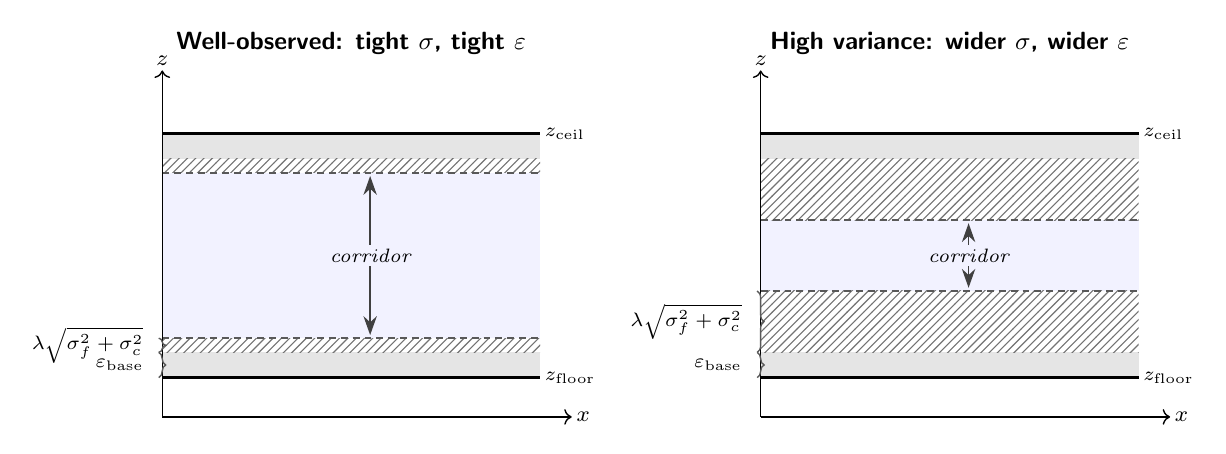
\begin{tikzpicture}[
    font=\footnotesize,
    every node/.style={inner sep=1.5pt},
    surface/.style={line width=1.0pt, draw=black},
    bound/.style  ={dashed, dash pattern=on 2.5pt off 1.8pt,
                    line width=0.55pt, draw=black!65},
    base/.style   ={fill=black!10, draw=none},
    var/.style    ={pattern=north east lines, pattern color=black!55,
                    draw=none},
    corridor/.style={fill=blue!5, draw=none},
    arr/.style    ={<->, >={Stealth[length=2.4mm,width=1.7mm]},
                    line width=0.55pt, draw=black!75},
    lbl/.style    ={font=\scriptsize},
    title/.style  ={font=\small\bfseries\sffamily},
    bracket/.style={decorate, decoration={brace, amplitude=2.5pt,
                                          mirror, raise=1pt},
                    line width=0.5pt, draw=black!65},
  ]

  %% --- common geometry --------------------------------------------------
  \def\W{4.8}     % panel width
  \def\H{4.0}     % axis top
  \def\zf{0.50}   % floor surface
  \def\zc{3.60}   % ceiling surface
  \def\eb{0.32}   % epsilon_base band thickness

  %% =====================================================================
  %% Panel 1: well-observed (small variance)
  %% =====================================================================
  \begin{scope}
    \def\sv{0.18} % variance-band thickness
    % corridor highlight (drawn first, behind everything)
    \fill[corridor] (0,{\zf+\eb+\sv}) rectangle (\W,{\zc-\eb-\sv});
    % epsilon_base bands at floor and ceiling
    \fill[base] (0,\zf) rectangle (\W,{\zf+\eb});
    \fill[base] (0,{\zc-\eb}) rectangle (\W,\zc);
    % variance bands (lambda*sigma) on top of epsilon_base
    \fill[var] (0,{\zf+\eb}) rectangle (\W,{\zf+\eb+\sv});
    \fill[var] (0,{\zc-\eb-\sv}) rectangle (\W,{\zc-\eb});
    % effective constraint boundaries
    \draw[bound] (0,{\zf+\eb+\sv}) -- (\W,{\zf+\eb+\sv});
    \draw[bound] (0,{\zc-\eb-\sv}) -- (\W,{\zc-\eb-\sv});
    % true surfaces (drawn after fills so they remain crisp)
    \draw[surface] (0,\zf) -- (\W,\zf);
    \draw[surface] (0,\zc) -- (\W,\zc);
    % surface labels on the right
    \node[lbl, anchor=west] at (\W,\zf) {$z_{\text{floor}}$};
    \node[lbl, anchor=west] at (\W,\zc) {$z_{\text{ceil}}$};
    % axes
    \draw[->, line width=0.5pt] (0,0) -- (\W+0.4,0)
          node[right, font=\footnotesize] {$x$};
    \draw[->, line width=0.5pt] (0,0) -- (0,\H+0.4)
          node[above, font=\footnotesize] {$z$};
    % corridor double arrow with inline label
    \draw[arr] ({\W*0.55},{\zf+\eb+\sv+0.04}) --
               ({\W*0.55},{\zc-\eb-\sv-0.04});
    \node[lbl, fill=blue!5, inner sep=1.5pt, font=\scriptsize\itshape]
          at ({\W*0.55},{(\zf+\zc)/2}) {corridor};
    % left-side brackets: epsilon_base, then lambda*sigma
    \draw[bracket] (-0.08,\zf) -- (-0.08,{\zf+\eb});
    \node[lbl, anchor=east] at (-0.18,{\zf+\eb/2}) {$\varepsilon_{\text{base}}$};
    \draw[bracket] (-0.08,{\zf+\eb}) -- (-0.08,{\zf+\eb+\sv});
    \node[lbl, anchor=east] at (-0.18,{\zf+\eb+\sv/2})
          {$\lambda\sqrt{\sigma_f^2+\sigma_c^2}$};
    % panel title
    \node[title, anchor=south] at ({\W/2},{\H+0.55})
          {Well-observed: tight $\sigma$, tight $\varepsilon$};
  \end{scope}

  %% =====================================================================
  %% Panel 2: high variance
  %% =====================================================================
  \begin{scope}[xshift=7.6cm]
    \def\sv{0.78}
    \fill[corridor] (0,{\zf+\eb+\sv}) rectangle (\W,{\zc-\eb-\sv});
    \fill[base] (0,\zf) rectangle (\W,{\zf+\eb});
    \fill[base] (0,{\zc-\eb}) rectangle (\W,\zc);
    \fill[var]  (0,{\zf+\eb}) rectangle (\W,{\zf+\eb+\sv});
    \fill[var]  (0,{\zc-\eb-\sv}) rectangle (\W,{\zc-\eb});
    \draw[bound] (0,{\zf+\eb+\sv}) -- (\W,{\zf+\eb+\sv});
    \draw[bound] (0,{\zc-\eb-\sv}) -- (\W,{\zc-\eb-\sv});
    \draw[surface] (0,\zf) -- (\W,\zf);
    \draw[surface] (0,\zc) -- (\W,\zc);
    \node[lbl, anchor=west] at (\W,\zf) {$z_{\text{floor}}$};
    \node[lbl, anchor=west] at (\W,\zc) {$z_{\text{ceil}}$};
    \draw[->, line width=0.5pt] (0,0) -- (\W+0.4,0)
          node[right, font=\footnotesize] {$x$};
    \draw[->, line width=0.5pt] (0,0) -- (0,\H+0.4)
          node[above, font=\footnotesize] {$z$};
    \draw[arr] ({\W*0.55},{\zf+\eb+\sv+0.04}) --
               ({\W*0.55},{\zc-\eb-\sv-0.04});
    \node[lbl, fill=blue!5, inner sep=1.5pt, font=\scriptsize\itshape]
          at ({\W*0.55},{(\zf+\zc)/2}) {corridor};
    \draw[bracket] (-0.08,\zf) -- (-0.08,{\zf+\eb});
    \node[lbl, anchor=east] at (-0.18,{\zf+\eb/2}) {$\varepsilon_{\text{base}}$};
    \draw[bracket] (-0.08,{\zf+\eb}) -- (-0.08,{\zf+\eb+\sv});
    \node[lbl, anchor=east] at (-0.18,{\zf+\eb+\sv/2})
          {$\lambda\sqrt{\sigma_f^2+\sigma_c^2}$};
    \node[title, anchor=south] at ({\W/2},{\H+0.55})
          {High variance: wider $\sigma$, wider $\varepsilon$};
  \end{scope}

\end{tikzpicture}
}
  \caption{The clearance margin $\varepsilon(x,y)$ tightens with map variance.}
  \label{fig:margin}
\end{figure}

where $\varepsilon_{\text{base}}$ absorbs irreducible factors (drill assembly extent, vibration amplitude, control tracking error) and $\lambda$ sets the confidence level. Under the Gaussian approximation that the per-cell Kalman update enforces, $\lambda = 3$ corresponds to a 99.7\,\% probability that the true clearance exceeds the estimated clearance minus the margin. This is the deterministic reformulation of the chance constraint $\Pr\bigl(c_{\text{true}}(x,y) \geq h_{\text{robot}} + \varepsilon_{\text{base}}\bigr) \geq 1 - \alpha$ with $\alpha = \Phi(-\lambda)$.

The margin then tracks the actual confidence of the underlying observations: it tightens at oblique LiDAR incidence, near the edge of the observed region, and on geometrically complex overhead features such as ducting, and relaxes towards $\varepsilon_{\text{base}}$ over flat, densely sampled ceiling surfaces. The constraint boundary moves with the map rather than with the worst case envisaged at design time.

None of the reviewed work on overhead clearance applies this principle. \citet{buchananWalkingPostureAdaptation2019} and \citet{DeformableConfigurationPlanning} use fixed scalar margins on dual-layer or deformable-bounding-box representations; the SubT stacks \citep{aghaNeBulaQuestRobotic2021,tranzattoTeamCERBERUSWins2024} statically inflate the volumetric occupancy field; \citet{mikiLearningWalkConfined2024} bypass an explicit margin by learning the policy directly. The asymmetry between the floor and ceiling layers is the open gap at the perception–constraint interface, and the variances needed to close it are already produced by a dual-layer Kalman-filtered map at no additional perception cost.

\subsection{Variable-geometry collision checking}
\label{sec:sq3:collision}

Standard mobile-robot collision checking treats the robot as a rigid footprint of fixed extent. For a platform whose geometry is itself a planning variable, the dual-layer perception of \Cref{sec:sq3:representation,sec:sq3:uncertainty} must be coupled to a parametric model of the configuration-dependent collision volume. The reviewed literature splits over three methodological commitments for entering the constraint: a parametric collision primitive queried against a clearance field, the reconfiguration variable embedded directly as a decision variable inside an optimiser, and search whose dimensionality varies with distance from the robot.

The first thread originates with \citet{buchananWalkingPostureAdaptation2019} on the hexapod Weaver. The robot is encased in an axis-aligned bounding box of fixed length and height, with a single parametric variable, the half-span, capturing the lateral extent as the leg pose changes; vertical clearance is checked by translating the box through $z$ via the legged platform's posture controller rather than by varying the box dimensions. The box is queried at a small set of points on its faces against a pair of robot-centric 2.5D elevation layers fused in the GridMap framework, and the resulting clearance margins drive a CHOMP trajectory optimiser. \citet{PerceptiveWholebodyPlanning} extend the same machinery to ANYmal at substantially greater body scale, demonstrating onboard mapping through 60~cm openings with end-to-end re-planning at roughly 500~ms. The reusable contribution is a parametric primitive plus a dual-layer clearance field consumed by a smoother; what does not generalise is the parameter choice, since a wheeled chassis with retractable limbs and a telescoping column exposes a different parametric variable governing vertical rather than lateral extent.

\citet{DeformableConfigurationPlanning} push the same primitive onto a parallel wheel-legged platform built around a Stewart-platform mechanism. The bounding box now has two free dimensions: trunk height and wheelbase are both treated as parameters, with the mechanical coupling (raising the trunk widens the support polygon) encoded through the parallel-mechanism Jacobian. Trajectory optimisation proceeds by covariant gradient descent against a signed distance field built offline from a fused, KD-tree-indexed point cloud. Three properties limit direct transfer: the distance field is pre-computed once from a static point cloud rather than maintained online; the safety margin is a fixed scalar rather than derived from the per-cell variance of \Cref{sec:sq3:uncertainty}; and on a Stewart platform trunk height and footprint are mechanically linked, whereas on a wheeled chassis with retractable limbs and a telescoping mast the column extension varies essentially independently of the planar footprint.

The second thread dispenses with the external collision primitive and exposes the reconfiguration variable to the optimiser itself. \citet{liAutonomousNavigationUnderactuated2023} present an end-to-end navigation framework for the bipedal robot Cassie. A vertically-actuated Spring-Loaded Inverted Pendulum (vSLIP) model captures the coupled dynamics of planar walking and walking height, and a three-layer planning hierarchy closes the loop: a global $A^{\star}$ search over a height-augmented graph penalising crouching depth proportional to the clearance deficit, a local vSLIP-based trajectory optimisation, and a hybrid-zero-dynamics controller tracking the variable-height reference. The transferable contribution is the treatment of the height variable as a first-class state in both the global graph and the local trajectory optimisation rather than as a parameter of an external primitive; the gait-stability machinery motivating the vSLIP reduction does not apply to a skid-steer base, so the planning-side abstraction transfers more readily than the dynamics-side one.

\citet{pankertDesignMotionPlanning2022} apply the same commitment on a wheeled mobile manipulator that switches between narrow-transit and wide-manipulation footprints. The reconfiguration variable enters the MPC directly alongside the planar pose, dispensing with the external collision primitive; this is the closest published instance of variable-geometry control on a wheeled platform inside an optimisation-based controller, treated at the planning-architecture level in \Cref{sec:sq4:reconfig}. Two limits qualify direct transfer: the variable is footprint width rather than vertical extent, and the leg references are supplied externally rather than driven internally by clearance-aware avoidance, so the optimiser trades reconfiguration against tracking error rather than against the perception-derived constraint surface that the platform under review requires.

The third thread, due to \citet{klamtPlanningHybridDrivingStepping2018} on the Momaro and Centauro platforms, varies the dimensionality of the search rather than the geometry of the robot. Near the current pose the search reasons over a high-dimensional state including foothold placement and individual wheel orientation; at larger distances it collapses to a coarser two-dimensional driveability representation with semantic annotations. The work is positioned for a discrete drive-versus-step mode switch rather than a continuous reconfiguration variable, and the height-augmented refinement is a property of the stepping mode rather than of the body geometry; the reusable principle is dimensionality-on-demand: configuration-dependent collision checking is paid for only where the robot is about to act, with the remainder of the search reduced to a planar problem.

Across the three threads, the reconfiguration variable enters the \emph{constraint surface} in three structurally different ways. How it enters the \emph{cost structure} of the planning problem is the question taken up in \Cref{sec:sq3:cost}.

\subsection{Reconfiguration cost formulation}
\label{sec:sq3:cost}

A planner that can vary the robot's height configuration must balance three competing objectives at every step of the prediction horizon: time-to-completion, ceiling clearance, and the cost of changing configuration. Sledge extension and limb adjustment are mechanically much slower than drive velocity, and any retraction-and-re-extension cycle inflates cycle time without contributing to forward progress. Synthesising the structure that recurs across the works reviewed below, the reconfiguration-aware path cost can be expressed as a weighted integral
\begin{equation}
J = \int_0^T \!\Bigl[\, w_t \;+\; w_c\, C_{\text{config}}(\dot{s}, \dot{h}_{\text{base}}) \;+\; w_m\, C_{\text{margin}}\!\bigl(c(x,y) - h_{\text{total}} - \varepsilon(x,y)\bigr) \,\Bigr]\, dt,
\label{eq:reconfig_cost}
\end{equation}
where $w_t$ penalises elapsed time, $C_{\text{config}}$ penalises configuration rates, and $C_{\text{margin}}$ penalises shortfall of the available clearance below the variance-aware threshold $\varepsilon(x,y)$ of \Cref{eq:probabilistic_margin}. No reviewed system presents this exact formulation; it is a generalisation that captures the common structure across the works below.

The closest published instance on a wheeled construction platform~\parencite{pankertDesignMotionPlanning2022} treats footprint reconfiguration as a decision variable in the MPC of a swerve-steering mobile manipulator with passively articulated legs. The cost, resolved at \SI{50}{\hertz} over a \SI{10}{\second} horizon, sums a base or end-effector tracking term, a leg-configuration tracking term $\lVert \varphi_L - \hat{\varphi}_L \rVert_2^2$, relaxed-barrier soft constraints, and a quadratic input penalty $u^\top R u$ over wheel, steering, leg, and arm rates; the leg-rate weight in $R$ is the direct analogue of $w_c$ on $\lVert \dot{h}_{\text{base}} \rVert^2$ in \Cref{eq:reconfig_cost}. The authors note that the leg references could in principle be optimised internally rather than supplied externally, in which case reconfiguration would be driven by collision avoidance rather than by a fixed schedule.

The legged NMPC lineage handles the analogous quantity on the swing foot. Foothold deviation from a Raibert heuristic is penalised with a quadratic regulariser on joint velocities~\parencite{grandiaPerceptiveLocomotionNonlinear2022}, suppressing changes of configuration that the trajectory does not require; whole-body wheeled-legged formulations~\parencite{bjelonic2021wholebody,sleiman2021unified} adopt the same template with input-rate weights distinguishing fast wheel rotations from slow leg or torso adjustments. Footholds enter the cost only at touchdown, a hybrid-timing structure, while the column extension considered here is a continuous state, so the resulting problem stays within standard input-rate-regularised receding-horizon control rather than the switched-system formulations of the legged literature. On the search-based side, a hybrid driving-stepping planner~\parencite{klamtPlanningHybridDrivingStepping2018} encodes the same trade-off as a discrete mode-switching cost where stepping primitives carry a substantially higher per-action cost than driving primitives, the discrete analogue of $w_c \gg w_t$ in \Cref{eq:reconfig_cost}.

What none of the reviewed instances captures is the dual role of the column variable. Sledge extension is at once a reconfiguration variable, which the running $w_c$ term should suppress in transit, and a task variable that must reach a per-target value $s_{\text{goal}}$ at every drill pose. The integral cost of \Cref{eq:reconfig_cost} alone cannot drive $s$ towards $s_{\text{goal}}$; capturing the dual role requires a terminal task cost
\begin{equation}
\Phi\bigl(\mathbf{x}(T)\bigr) \;=\; w_g \,\lVert s(T) - s_{\text{goal}} \rVert^2,
\label{eq:terminal_task_cost}
\end{equation}
active whenever the goal is a drill pose. The closest deployed industrial precedent, the Hilti Jaibot~\cite{hilti2020jaibot}, sidesteps the trade-off by enforcing $s = 0$ throughout all manually driven transit and reaching $s_{\text{goal}}$ only after coming to rest at each target, which in this cost vocabulary is a hard state constraint $s = 0$ in transit modes and is admissible but provably suboptimal whenever sustained partial extension would be safe. The variance-aware margin $\varepsilon(x,y)$ of \Cref{eq:probabilistic_margin} couples this trade-off back to perception: in well-observed regions the margin relaxes towards $\varepsilon_{\text{base}}$ and a planner can keep the column partially extended through tight clearances, while in regions of high map variance it tightens and forces conservative retraction.

\subsection{Discussion: a perception-coupled, variance-aware clearance gap}
\label{sec:sq3:discussion}

The four threads reviewed above each address part of the regime, none of them all of it. The two coupled commitments that no reviewed work makes jointly are: a margin that depends on the per-cell variance of both elevation layers, transporting the chance-constraint tightening established for the floor layer~\cite{fanSTEPStochasticTraversability2021,bipedal_cp_2025} (structurally identical to additive tightening in stochastic MPC~\cite{hewingLearningBasedModelPredictive2020,lorenzenConstraintTighteningStabilityStochastic2016}) to the overhead clearance constraint, despite the per-cell variance being available at no additional cost from the second elevation map instance~\cite{fankhauserProbabilisticTerrainMapping2018,mikiElevationMappingLocomotion2022}; and a cost structure in which the reconfiguration variable carries both a running-rate penalty and a terminal task value, capturing its dual role as transit-clearance variable and per-target task variable, where the closest wheeled instance~\cite{pankertDesignMotionPlanning2022} exposes the variable to the optimiser but supplies its tracking reference externally rather than driving it from a perception-derived clearance field. The integrated gap therefore lies at the intersection of the perception, collision-checking, and cost-formulation threads rather than within any one of them; the architectural choice between embedding the morphological state in a single optimal control problem and decomposing into a path-and-mode hierarchy is deferred to \Cref{sec:sq4}.

\section{SQ4: Planning architectures for ceiling-constrained navigation}
\label{sec:sq4}

A platform whose collision volume is itself a planning variable must coordinate a planar trajectory with a configuration profile under hard overhead clearance constraints derived from online perception. This section reviews the planning and control architectures available for this coupled problem, organised by their progression from layered-costmap navigation stacks, through search- and optimisation-based receding-horizon control, to reactive and learning-based approaches.

\subsection{Standard navigation stacks}
\label{sec:sq4:navstacks}

The dominant paradigm for ground-robot navigation in the ROS ecosystem is the layered-costmap stack~\parencite{luLayeredCostmapsContextsensitive2014}. A global planner operates on a single 2D master costmap whose per-cell value is fused from a stack of plugin layers (static, obstacle, inflation, voxel, semantic), and a local controller tracks the resulting path while reacting to dynamic returns. The ROS\,2 reimplementation Nav2~\parencite{macenski2020nav2} follows this pattern with a plugin-based planner, controller, and recovery architecture, and the Smac Planner~\parencite{macenskiOpenSourceCostAwareKinematically2025} provides high-performance Cost-Aware A*, Hybrid-A*, and State Lattice variants for kinematically feasible search over arbitrary-footprint platforms, building on the differentially constrained lattice formulation~\parencite{pivtoraikoDifferentiallyConstrainedMobile2009}. Nav2 also exposes the GPU-parallel MPPI controller~\parencite{williamsAggressiveDrivingModel2016} as a controller plug-in, reviewed in \Cref{sec:sq4:mppi}.

Two structural properties of the layered-costmap design block overhead-constrained navigation. First, the master costmap is a single 2D grid. Layers may consume 3D sensor data internally (the \texttt{VoxelLayer} and the spatio-temporal voxel layer maintain volumetric occupancy buffers), but each writes a 2D scalar cost into the master through a fixed reduction. The column projection is bounded by \texttt{min\_obstacle\_height} and \texttt{max\_obstacle\_height} parameters set at launch; neither tracks a configuration variable. A cell is therefore either lethal or free for the planner regardless of whether the platform is in a tall or compact configuration. Second, the architecture provides no mechanism for fusing layers under a configuration-dependent rule: the only available reductions are pixel-wise maximum, sum, or override. Approximating overhead awareness within this framework leaves two options, both unsatisfactory. Inflating the costmap to the worst-case height envelope is over-conservative; it excludes regions passable when the platform is retracted. Precomputing one costmap per discrete height level discretises a continuous degree of freedom and still leaves path and height to be optimised separately.

\subsection{Search-based planning with height augmentation}
\label{sec:sq4:search}

Search-based planners can in principle accommodate additional state dimensions by augmenting the search graph. The state lattice formulation~\parencite{pivtoraikoDifferentiallyConstrainedMobile2009} is a regular sampling of the configuration space whose edges are precomputed motion primitives encoding the platform's differential constraints, so that any path returned by graph search over the lattice is by construction kinematically feasible. The Smac Planner~\parencite{macenskiOpenSourceCostAwareKinematically2025} provides the open-source implementation in $(x, y, \theta)$, with a minimum control set computed offline, cost-aware A$^{\star}$ over the resulting graph, and arbitrary-footprint collision checking against a 2D costmap discretised at the grid resolution. This is the global planner currently in operational use on the platform under study for floor-only navigation.

Extending the lattice to $(x, y, \theta, s)$ by adding a discretised reconfiguration variable is straightforward in principle and computationally costly in practice. The branching factor scales multiplicatively in the number of height levels, the control set must be regenerated to include coupled drive-and-reconfiguration primitives at every discretised value of $s$, and the heuristic must capture both planar progress and reconfiguration cost without losing admissibility. A centimetre-scale discretisation against the column travel of the platform considered here would multiply the lattice by two orders of magnitude, while a coarse three-level discretisation (retracted, mid, extended) excludes the partially-extended trajectories that are precisely the regime where joint optimisation of path and configuration pays off.
% \begin{comment}
% Thesis restoration: the original lit-study draft carried the explicit
% NDA-sensitive figure: "of order centimetres against roughly 1.3~m of
% mast travel". Restore the explicit ratio once NDA constraints lift.
% \end{comment}

The principled response in the literature is dimensionality-on-demand. Planning with adaptive dimensionality~\parencite{gochev2011adaptive,gochev2013incremental} constructs a low-dimensional graph by default and introduces high-dimensional regions only where the low-dimensional plan would otherwise be infeasible, with a guarantee that the recovered solution is feasible in the original high-dimensional space; reported planning-time reductions of one to two orders of magnitude over a uniformly high-dimensional search on mobile-manipulation problems. The hybrid driving-stepping planner~\parencite{klamtPlanningHybridDrivingStepping2018}, treated at the collision-check level in \Cref{sec:sq3:collision}, applies the same principle on a wheeled-legged platform: in the immediate vicinity of the robot the search reasons over a high-dimensional state including foothold placement and individual wheel orientation, while at larger distances it collapses to a coarser two-dimensional driveability representation enriched with semantic annotations. The reusable principle is that configuration-dependent collision checking is paid for only in the region of the workspace where the robot is about to act, with the remainder of the search reduced to a planar problem.

The closest published instance of a search-based planner that consumes a dual-surface representation is the four-dimensional planner of \texttt{ugv\_nav4d}~\parencite{bockmannUgv_nav4dAdvancedMultiSurface2024}, reviewed at the representation level in \Cref{sec:sq1:mls}. SBPL ARA$^{\star}$ runs over $(x, y, z, \theta)$ with motion primitives matched to a wheeled platform's kinematic envelope, where the third dimension captures the surface index of a multi-level surface map rather than a morphological reconfiguration variable. The architectural pattern is directly relevant: a graph search over the augmented state with motion primitives precomputed to respect the kinematic and surface-transition constraints of the underlying representation. Two elements qualify direct transfer at the planning-architecture level. The traversability map has to be expanded from the underlying multi-surface representation before each planning cycle rather than queried continuously, which fixes the planner's role as a periodic global planner rather than a closed-loop controller; and the augmented dimension encodes a discrete surface choice rather than the continuous configuration variable that the platform under study exposes.

Two related search-based threads sit closer to a height-augmented formulation but each handles the height variable differently. The Point Cloud Tomography planner~\parencite{yangEfficientGlobalNavigational2024} runs a modified A$^{\star}$ search over a stack of horizontal tomograms and connects adjacent slices through gateway cells, the same planar position appearing in an adjacent slice with lower cost above or below; the resulting waypoint sequence is post-processed by a polynomial optimisation that adjusts the body height $q_z(t)$ between the ground and ceiling layers. The height variable is therefore handled outside the lattice search itself rather than inside it, and the slice gateways re-introduce the same per-cell discontinuities flagged at the representation level. A bipedal-walker formulation~\parencite{liAutonomousNavigationUnderactuated2023} keeps height as a first-class search dimension by handing a height-augmented A$^{\star}$ output to a vSLIP-based local trajectory optimiser that closes the gait dynamics, and reports admissible-height penalties proportional to clearance deficit; the bipedal reduction does not transfer to a wheeled chassis whose drive dynamics are simpler than a walking gait.

Two structural properties of any search-based augmentation are independent of the specific dimensionality strategy and bear on the comparison with the receding-horizon architectures considered in the following subsections. First, the output of a lattice search is a sequence of grid-aligned waypoints without explicit trajectory timing, so a downstream controller must generate dynamically feasible motion that tracks both the planar reference and the reconfiguration profile. Second, the resolution-versus-tractability trade-off is reduced under adaptive dimensionality but not eliminated, and the per-cell discontinuities that arise at lattice cell boundaries and at any switching between dimensionality levels remain incompatible with the C$^{1}$-smooth constraint fields that the gradient-based controllers reviewed below consume. A search-based augmentation is therefore a viable global-planning stage but not, on the present evidence, a viable closed-loop controller in its own right for a platform whose effective collision volume must track a continuous reconfiguration variable at control-loop rate.

\subsection{Sampling-based model predictive control}
\label{sec:sq4:mppi}

Model Predictive Path Integral (MPPI) control~\parencite{williams2017infomppi,williams2018infomppi} is a free-energy-weighted average over Monte Carlo trajectory rollouts under the system dynamics. The formulation needs neither convexity nor analytic constraint Jacobians and admits non-smooth and non-differentiable cost terms, which gradient-based NMPC handles only after substantial smoothing. Thousands of parallel rollouts per cycle map efficiently to GPU and, more recently, to multi-core CPU. MPPI is also the local trajectory optimiser currently in operational use through the Nav2 controller plugin interface on the platform considered in this work.

Standalone MPPI has a structural limitation in safety-critical regimes. Hard inequality constraints enter only as cost penalties, and a finite Monte Carlo sample certifies no drawn trajectory as feasible. Sampling fails most often near the constraint boundary, where the feasible control-sequence volume shrinks below the coverage of a fixed-variance Gaussian sampler. For a platform required to navigate within centimetres of an overhead surface to exploit clearance margin, this failure mode applies directly.

Shield-MPPI~\parencite{yin2023shieldmppi} is the family-defining safety-augmented variant: a discrete-time Control Barrier Function (DCBF) penalty added to the running cost biases the sampler towards feasible trajectories without altering the parallel rollout structure, after which the weighted-average control sequence passes through a local gradient-repair step that minimises residual DCBF violations on the committed control. The construction reduces constraint violations by an order of magnitude on the AutoRally aggressive-driving platform with sample counts an order of magnitude below unaugmented MPPI, which weakens the family's dependence on dedicated GPU compute, the binding resource in the embedded regime of \Cref{sec:sq6}. Three follow-ups extend the template along orthogonal axes: learned neural CBFs for input-constrained systems where the high-relative-degree analytic construction is non-trivial~\parencite{so2025nsmppi}, augmented-state BR-MPPI that lifts the class-$\mathcal{K}$ parameter into the controlled state to convert the CBF inequality into a sampled equality~\parencite{parwana2025brmppi}, and a value-function-based Robust Policy CBF that admits bounded disturbances and high relative degree~\parencite{knoedler2025rpcbf}.

A safety-augmented MPPI architecture that consumes the clearance field of \Cref{sec:sq3} as the barrier function $B(\mathbf{x}) = f(x, y, s)$ would extend the existing Nav2 MPPI integration with hard ceiling-constraint enforcement through one of the constructions reviewed above. The structural trade-off relative to the NMPC architectures of \Cref{sec:sq4:nmpc} is when the safety guarantee fires. The DCBF penalty enters the rollout cost over the prediction horizon and biases the samples predictively, but the formal guarantee comes from the local repair step, which sees only the current state and acts on a single committed control. On a platform whose configuration variable couples to the constraint boundary over several seconds of sledge actuation, with a margin that varies along the executed path, the repair step cannot discover that routing around an overhead obstacle is globally faster than retracting through it. The controller enforces safety at every step but does not optimise the height profile over the receding horizon as a coupled trajectory.

\subsection{Nonlinear model predictive control for navigation}
\label{sec:sq4:nmpc}

Nonlinear model predictive control (NMPC) merges the global-planning and local-tracking layers of \Cref{sec:sq4:navstacks} into a single online optimal control problem. At each cycle the controller optimises a finite-horizon trajectory under dynamics, input bounds, and inequality constraints; commits the first input of the optimal sequence; and re-solves at the next cycle warm-started from the previous solution. Two structural commitments distinguish the gradient-based variant from the sampling-based controllers of \Cref{sec:sq4:mppi}. Every term entering the constraint set must be at least $C^1$-smooth so that the QP subproblem is well-posed and Jacobians are computable, which dictates the representations admissible at the perception layer and the field formulations admissible at the clearance layer (\Cref{sec:sq1,sec:sq3}). The cost gradient must propagate cleanly through the model, which favours analytically differentiable kinematic descriptions over learned dynamics. Embedded SQP-type solvers with template kernel libraries now reach single-digit-millisecond cycles on ARM-class hardware for moderate problem sizes, reviewed at the deployment level in \Cref{sec:sq6}.

\citet{grandiaPerceptiveLocomotionNonlinear2022} demonstrate the perception-to-NMPC interface on a quadrupedal platform. A robot-centric elevation map is preprocessed into three constraint primitives consumed by the optimiser at each cycle: a per-cell steppability score, a connected-component plane segmentation that supplies polytopic foothold inequalities, and a signed distance field with analytic gradients for body and swing-leg avoidance. Each abstraction is wrapped in a relaxed log-barrier so that polytope edges and SDF zero-crossings preserve the smoothness the family demands. The system is the floor-only template for online perception-driven NMPC; extension to a second mapped surface is a representation requirement raised by \Cref{sec:sq1}, not a controller property inherited from the floor case.

\citet{gaertnerCollisionFreeMPCLegged2021} take the same platform but a different question: collision-free whole-body locomotion under static and dynamic obstacles. The controller evaluates a relaxed barrier on a dynamically generated Euclidean SDF of the static scene, with explicit checks against moving cylinders for dynamic agents and a Kalman-filter motion prediction supplying their receding-horizon trajectory. The reported behaviour includes automatic crouching under low overhead obstacles without any heuristic switching: the cost gradient discovers through the kinematic chain that lowering the torso reduces the barrier penalty by more than the locomotion cost it incurs. The class-level property is that configuration enters the constraint surface through the model itself rather than through an external scheduler or a switched policy. The platform considered here exhibits the same property through a prismatic mast variable governing vertical extent rather than a swing-leg variable governing posture, a kinematic class on which this construction has not been demonstrated.

\citet{kohlerMPCFrameworkEfficient2025} address a structural limitation of the receding-horizon paradigm at the global-planning interface: a standalone NMPC over a finite horizon stalls in local minima whenever the detour to the target exceeds the horizon. The proposed framework embeds a finite-segment shortest-path planner directly inside the MPC, optimising jointly the dynamic trajectory and a kinematics-free path from its terminal state to the target, initialised by Dijkstra search over a visibility road map. The combined scheme inherits stability, convergence, and collision-avoidance guarantees for arbitrary nonlinear dynamics in cluttered environments, validated on a small wheeled platform. The mechanism delegates topological reachability to a search-based stage and leaves dynamics and constraint enforcement to the receding-horizon controller, a structural division any NMPC operating beyond its single-horizon range must adopt in some form.

\citet{jacquet2025sdfnmpc} take the perception-to-NMPC interface to a learned representation. A neural model compresses a single onboard range image into a continuous, differentiable three-dimensional signed distance function, evaluated as an explicit position inequality at each shooting node of an online NMPC. The full multirotor velocity-tracking problem, augmented with field-of-view constraints, runs at approximately \SI{10}{\milli\second} per cycle on onboard compute, with recursive feasibility and stability guarantees holding under fixed observations. The class-level evidence is that perception-derived continuous distance fields are now consumable as differentiable inequalities inside an embedded NMPC, with the learning machinery contained on the perception side rather than in the controller.

Across these instances, gradient-based NMPC supplies hard inequality enforcement against smooth perception-derived fields, with the finite-horizon local-minimum issue as the standing limitation of the family. Two architectural responses close it: an external search-based stage in the manner of \citet{kohlerMPCFrameworkEfficient2025}, or a hierarchical decomposition into a planning layer and a tracking layer, reviewed next. The application of either response to a wheeled chassis whose effective collision volume varies with a continuous configuration variable is not on record.

\subsection{Hierarchical model predictive control}
\label{sec:sq4:hmpc}

A complementary response to the planning-horizon-versus-sampling-rate trade-off that constrains a single-level NMPC on embedded hardware is to split the receding-horizon problem across two layers: a slow Planning MPC (PMPC) over a long horizon, supplying a reference trajectory to a fast Tracking MPC (TMPC) over a short horizon. Hierarchical MPC (HMPC) of this form has been studied for two decades, with most early instances using a reduced-order linearised model in the upper layer to recover real-time tractability~\cite{farina2017hierarchical,raghuraman2022adjustable}, at the cost of restricting the manoeuvres the planner can express. The obstacle to embedded deployment has been the co-design problem: the PMPC must produce a reference that the TMPC is provably able to track, with constraint tightening that absorbs both model mismatch and the bounded tracking error of the lower layer.

An embedded HMPC framework~\parencite{bendersEmbeddedHierarchicalMPC2025} resolves the co-design problem for mobile robots while retaining the same nonlinear model in both layers. The TMPC is designed first against the original system constraint set $\mathcal{Z} = \{(x,u) \mid g_j^s(x,u) \leq 0, \ j \in \mathbb{N}_{[1,n^s]}\}$ and the original free-space set $\mathcal{F}_{\tau|t}$, with offline-computed terminal cost, terminal control law, and terminal set such that closed-loop tracking error remains within a positive invariant tube of scaling $\alpha$. The PMPC is then formulated against the same nonlinear dynamics but with each constraint tightened by a constant $c_j \cdot \alpha$ derived from the projection of the tube onto the constraint normal:
\begin{equation}
g_j^s(x,u) \leq -c_j^s \alpha, \qquad L_{j,\tau|t}^o p_{\tau|t} \leq l_{j,\tau|t}^o - c_j^o \alpha.
\end{equation}
The two theorems of the paper prove that this construction yields recursive feasibility of the joint scheme and closed-loop collision avoidance, under static obstacles and bounded disturbances. The reported quadrotor implementation, with both layers solved by an acados SQP-RTI scheme on the onboard computer, achieves a planning horizon five times longer than a single-layer NMPC at the same compute budget, with the open-source code released alongside the paper.

The obstacle avoidance interface is a sequence of overlapping convex polytopes generated online by the I-DecompUtil library~\parencite{liu2017sfc}. Starting from a piecewise-linear path produced by a fast graph search, the algorithm grows axis-aligned ellipsoids around each segment until they meet the nearest occupied cell, and the dual halfspace representation $L^o p \leq l^o$ of each ellipsoid yields a Safe Flight Corridor of overlapping convex polyhedra. Each PMPC stage is associated with one polytope of the corridor, and the obstacle avoidance constraint at that stage reduces to a small set of linear inequalities that pass directly into the QP backend.

Three properties of this architecture bear on the platform regime under review. First, the polytopic constraint structure aligns with the output of plane-segmentation pipelines~\cite{schoels2020convex_decomp,erniMEMMultiModalElevation2023}: each ceiling plane segmented from a 2.5D ceiling layer, and each floor corridor extracted from the traversability costmap, is a halfspace inequality the PMPC accepts directly. Second, the two-layer rate hierarchy maps onto the dual-rate sensing of \Cref{sec:sq1}: the PMPC can refresh its corridor at the elevation map update rate of \SIrange{5}{10}{\hertz}, while the TMPC closes the loop on the drive controller at $\geq$\SI{20}{\hertz} against measurements that need not wait for the perception cycle. Third, recursive feasibility supplies a property no other architecture reviewed in this section provides: once a feasible plan with a specific configuration profile has been committed by the PMPC, the TMPC is proven to maintain feasibility under bounded disturbances throughout execution, without the runtime infeasibility recoveries that single-layer NMPC must rely on heuristics to handle.

Three structural extensions remain to be developed before the framework can apply to a wheeled platform whose collision volume is itself a planning variable. First, the published instance handles a six-degree-of-freedom rigid body whose obstacle avoidance reduces to a position constraint $p \in \mathcal{F}_{\tau|t} \subset \mathbb{R}^3$; encoding overhead clearance against a configuration variable requires augmenting the constraint set with mixed-dimension inequalities, spatial halfspaces in the planar position $(x,y)$ together with halfspaces in the morphological state $s$ that couple the two through the floor-ceiling clearance field of \Cref{sec:sq3}. Second, the interaction of mixed-dimension constraints with the constant-tightening scheme has not been studied within this lineage, and the relevant disturbance set is anisotropic because the actuator bandwidths governing the planar dynamics and the morphological states differ by more than an order of magnitude; separate tightening constants per constraint group, derived from the projection of an anisotropic disturbance invariant set onto each constraint normal, are the natural extension but require an offline terminal-ingredient computation that has no published precedent for this regime. Third, I-DecompUtil itself generates a planar corridor; the dual-surface decomposition that pairs a floor corridor with a stack of ceiling halfspaces sharing the $(x,y,s)$ coupling is not part of the published library and would be built alongside the controller.

The framework is therefore a candidate, not a deployed solution, for the planning problem treated in this review. Its formal guarantees on recursive feasibility are the strongest available for embedded receding-horizon control with hard obstacle constraints; the extensions enumerated above remain to be developed.

\subsection{Reconfigurable robot planning}
\label{sec:sq4:reconfig}

Variable-geometry collision checking, reviewed in \Cref{sec:sq3}, establishes that morphological state can be exposed to a planner; the architectural question is where in the planning hierarchy the resulting decision variable lives. Three positions appear in the literature. The first keeps reconfiguration outside the closed-loop controller, with a sampling-and-smoothing pipeline producing a body-pose trajectory that deforms against a signed distance field built from dual elevation layers, the configuration profile emerging as a property of the deformed trajectory rather than as a committed decision variable~\cite{buchananWalkingPostureAdaptation2019,PerceptiveWholebodyPlanning}. The second exposes reconfiguration to a search-based planner as a discrete mode-switching cost, with categorical modes (drive versus step, footprint dimensions) whose per-action costs bias the search and produce a sequence of mode-switch waypoints rather than a continuously adjustable trajectory~\cite{klamtPlanningHybridDrivingStepping2018,raghavanAgileLeggedWheeledReconfigurable2020}. The third exposes the morphological variable directly as a decision variable in a receding-horizon controller: \citet{pankertDesignMotionPlanning2022} include the leg-configuration variables of a swerve-steering mobile manipulator in a unified MPC alongside the planar pose, wheel rates, and manipulator joints, traded against tracking error through input-rate penalties on slow leg and fast wheel actuators. This is the closest published instance of variable-geometry control on a wheeled platform inside an optimisation-based controller, but with leg references supplied externally and the variable footprint span rather than vertical extent.

What remains open is the third position instantiated for a wheeled platform whose effective height varies through discrete mechanical reconfiguration: a continuous reconfiguration variable driven internally by the perception-derived clearance representation rather than tracked from an external reference or gated by a static collision primitive, on a chassis whose vertical extent is supplied by a single prismatic mast. The architectural verdict among the controller families that admit this placement is taken up in \Cref{sec:sq4:discussion}.

\subsection{Discussion: architectural gap and design space}
\label{sec:sq4:discussion}

The architectures reviewed in this section address the planning problem from structurally different positions. Standard navigation stacks~\cite{luLayeredCostmapsContextsensitive2014,macenski2020nav2,macenskiOpenSourceCostAwareKinematically2025} treat the platform as a fixed-footprint shape and admit no rule under which a configuration variable enters; search-based augmentation~\cite{gochev2011adaptive,bockmannUgv_nav4dAdvancedMultiSurface2024,yangEfficientGlobalNavigational2024,liAutonomousNavigationUnderactuated2023} restores the vertical dimension at the cost of grid-aligned, untimed waypoints with discontinuities at cell boundaries. Sampling-based receding-horizon control~\cite{williams2017infomppi} accommodates non-smooth and learnt costs but provides no formal certificate that any drawn trajectory satisfies an inequality. Gradient-based receding-horizon control~\cite{grandiaPerceptiveLocomotionNonlinear2022,gaertnerCollisionFreeMPCLegged2021,jacquet2025sdfnmpc,kohlerMPCFrameworkEfficient2025} supplies hard constraint enforcement against smooth perception-derived fields but no inherent recursive feasibility, and hierarchical receding-horizon control~\cite{bendersEmbeddedHierarchicalMPC2025} adds that guarantee under bounded disturbances at the cost of a co-design problem and an offline terminal-ingredient computation.

Three further families (optimisation fabrics~\cite{spahn2023fabrics,spahn2025implicit,merva2025g3f}, reinforcement-learning policies~\cite{xuDexterousLeggedLocomotion2024,mikiLearningWalkConfined2024,freyLocomotionPolicyGuided2022}, and diffusion-based trajectory generators~\cite{yan2025m2diffuser,cao2025dare,chi2023diffusionpolicy}) are well posed in their own deployment regimes but fail the hard-constraint filter formalised below: fabrics make no formal constraint-satisfaction guarantee with reported collisions arising from numerical integration error and local minima at vanishing terminal velocity, and RL and diffusion encode avoidance through reward shaping or learnt score gradients rather than as inequalities the policy is provably forbidden from violating. The diffusion thread additionally fails the embedded filter at present: desktop-class GPU latencies of order \SI{0.1}{\second} per query~\cite{chi2023diffusionpolicy} that recent one-step and few-step accelerations have not yet demonstrated within the unified-memory budget of an embedded GPU under concurrent perception workloads. All three are retained as future-work directions, not as primary controller candidates; fabrics in particular remain a candidate inner safety layer subordinate to one of the optimisation-based architectures of \Cref{sec:sq4:nmpc,sec:sq4:hmpc}.

Two structural filters narrow the design space. Gradient-based controllers consume constraint fields that are at minimum $C^1$-smooth, which excludes search-based and multi-level surface representations as primary closed-loop controllers; they remain viable as periodic global-planning stages feeding a downstream receding-horizon controller. A regime in which the consequence of constraint violation is collision between a drill assembly and reinforced concrete excludes architectures whose only safety mechanism is cost penalty or reward shaping. Three architectures survive both filters: gradient-based receding-horizon control against smooth perception-derived fields, hierarchical receding-horizon control with polytopic constraint tightening, and sampling-based receding-horizon control with a control-barrier-function safety filter on the committed control. \Cref{tab:sq4_comparison} consolidates how each family scores against the requirements the platform under review imposes.

\begin{table}[t]
\centering
\caption{Comparison of planning architectures against the requirements imposed by a wheeled platform with reconfigurable height under online-mapped overhead constraints.}
\label{tab:sq4_comparison}
\footnotesize
\setlength{\tabcolsep}{4pt}
\renewcommand{\arraystretch}{1.15}
\begin{tabularx}{\linewidth}{@{}l *{5}{>{\centering\arraybackslash}X}@{}}
\toprule
             & Height as     & Hard ceiling & Recursive    & Global    & Embedded    \\
Architecture & decision var. & constraints  & feasibility  & guidance  & feasibility \\
\midrule
Nav2 (SMAC + MPPI)        & \ding{55} & \ding{55} & \ding{55} & \ding{51} & \ding{51} \\
4D state lattice          & \ding{51} & \ding{51} & \ding{55} & \ding{51} & ? \\
Single NMPC               & \ding{51} & \ding{51} & \ding{55}\textsuperscript{$\dagger$} & \ding{55}\textsuperscript{$\ddagger$} & \ding{51} \\
HMPC (PMPC + TMPC)        & \ding{51} & \ding{51} & \ding{51} & \ding{51} & \ding{51} \\
CBF-augmented MPPI        & \ding{51} & \ding{51}\textsuperscript{$\S$} & \ding{55} & \ding{55}\textsuperscript{$\ddagger$} & \ding{51} \\
Geometric fabrics         & \ding{51} & \ding{55} & \ding{55} & \ding{55} & \ding{51} \\
RL policy                 & \ding{51} & \ding{55} & \ding{55} & \ding{55} & \ding{51} \\
Diffusion policy          & \ding{51} & \ding{55} & \ding{55} & \ding{55} & \ding{55}\textsuperscript{$\|$} \\
\bottomrule
\end{tabularx}

\smallskip
{\footnotesize\raggedright
\textsuperscript{$\dagger$}\,Recursive feasibility can be added through constraint tightening but is not inherent in a single-level NMPC.\\
\textsuperscript{$\ddagger$}\,No inherent global planning; can be supplied externally by a search-based reference-path source.\\
\textsuperscript{$\S$}\,Hard constraints enforced reactively by the CBF safety filter, not predictively over the horizon.\\
\textsuperscript{$\|$}\,Diffusion samplers currently require workstation-class GPUs; recent acceleration work is not yet demonstrated on embedded GPUs under concurrent perception load.\par
}
\end{table}

The architecture-level gap is the absence of an architecture that simultaneously admits the morphological reconfiguration variable as a continuous decision variable rather than as a discrete graph dimension, external reference, or emergent policy output; enforces overhead clearance as a hard constraint against a perception-derived field rather than as a cost penalty, soft barrier, or reward-shaping term; consumes the dual-layer constraint field of \Cref{sec:sq3} with the variance-aware tightening of \Cref{sec:sq3:uncertainty} transported from the perception layer; and executes within the unified-memory and latency envelope of \Cref{sec:sq6} under concurrent perception workloads. The choice between the three surviving families is deferred to \Cref{sec:proposed-methodology}: the components are individually mature, but their combination on the platform regime considered is undocumented, and the relative weight of formal guarantees, predictive optimality, embedded latency under shared-memory GPU contention, and implementation complexity cannot be resolved from the published evidence alone.

\section{SQ5: Positioning and goal selection}
\label{sec:sq5}

A platform that drills overhead targets must, for each target, choose a base pose and morphological configuration from which the drill end-effector can reach the target in the required orientation. This section reviews the mobile-manipulation literature on workspace representation and base placement, organised by its progression from forward capability maps through inverse reachability maps, cost-aware and uncertainty-aware placement strategies, learning-based alternatives, and the BIM-driven construction-robotics literature in which an overhead drilling task is the deployment regime.

\subsection{Reachability and capability maps}

The capability map~\parencite{zacharias2007capturing} is a 6D voxel grid of the manipulator workspace in which each voxel stores a scalar reachability index together with a directional structure capturing which end-effector orientations remain feasible at that position. The voxel score extended Yoshikawa's manipulability ellipsoid with joint-limit and self-collision factors. The journal version~\parencite{zacharias2013capability} extended the construction to redundant arms and standardised the data layout adopted by subsequent open-source tooling. A consolidated analysis~\parencite{ReachabilityCapabilityAnalysis2025} across grasp selection, path planning, and workcell layout establishes the capability map as the dominant offline representation of arm dexterity.

A capability map answers the \emph{forward} question: from a given base pose, which end-effector poses are reachable? For mobile manipulators the relevant question is the \emph{inverse}: given a desired task pose, which base placements are kinematically valid?

\subsection{Inverse reachability maps}

Inverse reachability maps (IRMs)~\parencite{RobotPlacementBased} formalise base-pose selection by transforming each cell of a precomputed capability map into the base frame, yielding a distribution in SE(2) scored by the inherited manipulability index. A humanoid extension~\parencite{burget2015stance} replaces the planar base distribution with a foothold-pose distribution that respects support-polygon constraints. In both formulations placement is selected by sampling from a precomputed distribution, with candidate quality read off the map without an online inverse-kinematics call.

The open-source \textsc{Reuleaux} package~\parencite{makhalReuleauxRobotBase2017} constructs both forward and inverse maps for arbitrary URDF-specified manipulators. RM4D~\parencite{rudorferRM4DCombinedReachability2024} reduces the discretisation from 6D to 4D by exploiting full rotation of the first and last joints on most commercial 6- and 7-axis arms, serving both forward and inverse queries from a single data structure. An oriented-surface generalisation~\parencite{birrOrientedSurfaceReachability2022} extends the placement target from a single horizontal support plane to arbitrarily oriented planes in 3D space, with a height-map segmentation extracting planar regions in Hessian normal form against which the IRM is queried. A more recent formulation~\parencite{cavelliMobileManipulatorBase2025} replaces workspace discretisation with two concentric ellipsoids fitted to a kinematic point-cloud sample, supporting analytical base-placement optimisation at the cost of the directional information that discretised representations preserve.

\subsection{Cost-aware placement and task sequencing}

Classical IRMs identify \emph{feasible} base poses but do not rank them by cost. A time-efficient placement objective~\parencite{reisterCombiningNavigationManipulation2022} combines a navigation cost (time to drive between consecutive base poses) with a manipulation cost (an extended manipulability index sourced from an inverse reachability map), validated in simulation and on a humanoid platform clearing a table. The structural pattern, a planar-motion cost summed with a quality term keyed to the IRM, is platform-agnostic and applies wherever a mobile manipulator must rank reachable base poses.

When a mission involves multiple targets, task sequencing becomes relevant. The mobile-manipulator Robotic Task Sequencing Problem has been formulated~\parencite{nguyenTaskSpaceClusteringMobile2023} as a Set Cover problem on a bipartite graph that links targets to candidate base poses by reachability, then sequences motion across the resulting clusters. The framework is validated on a mobile drilling experiment with several hundred targets, the closest published deployment regime to multi-hole ceiling-drilling campaigns, and outperforms prior sequencing methods in solution quality at comparable compute cost. Neither construction couples the inter-target cost to the geometry traversed between targets, a limitation taken up in \Cref{sec:sq5}.

\subsection{Placement under uncertainty}

Real-world positioning is subject to localisation error, which can render a nominally feasible IRM cell infeasible at execution time. An inscribed-disc formulation~\parencite{xu2020planning} addresses this by selecting placements at the centre of the largest disc inscribable in the intersection of consecutive feasibility regions, requiring the disc radius to exceed the expected positioning error. A non-convex generalisation~\parencite{gautierOptimizingRobotPositioning2025} extends the principle through particle-swarm exploration, with a Voronoi-based inscribed-circle radius as the robustness criterion. On a skid-steer platform the relevant error envelope is dominated by wheel-slip-induced odometry drift.

\subsection{Learning-based placement}

Learning-based methods replace or augment static reachability maps with predictions fitted from interaction data. A hybrid actor-critic framework~\parencite{jauhriRobotLearningMobile2022} retains the IRM as a behaviour prior, regularising both the policy and the value function, with zero-shot sim-to-real transfer. A graph-neural-network extension~\parencite{naik2024basenet} addresses multi-target sequencing by jointly selecting per-target base poses and visit order, halving combined planning and execution time relative to combinatorial-optimisation baselines. A hierarchical world-model formulation~\parencite{fengPredictiveReachabilityEmbodiment2024} replaces the offline IK test that gates base-to-arm transitions with embodiment switching from image observations alone, removing the offline-IK dependency the preceding threads inherit. None demonstrates transfer beyond the simulator and reward stack used for training.

\subsection{Construction robotics: BIM-driven positioning}

In construction settings, target poses are typically derived from Building Information Models (BIM). The Hilti Jaibot~\citep{hilti2020jaibot}, a semi-autonomous ceiling-drilling robot commercially deployed since 2020, consumes BIM-defined drill coordinates and uses a robotic total station (PLT~300) for indoor positioning. An operator drives the platform to an approximate location, after which the arm drills all reachable holes within a fixed working radius; no autonomous base-placement optimisation is performed. A 2022 firmware update added on-board sensing of corrugated metal-deck profiles to adapt planned holes to as-built deviations, an acknowledgement that the model alone is insufficient at the tolerances overhead drilling requires.

\citet{kimDevelopmentBIMintegratedConstruction2021} develop an IFC-to-SDF converter that exposes BIM geometry to ROS-based Gazebo simulation, demonstrated on indoor wall painting; the work targets the BIM-to-simulation interface and does not address base-placement optimisation. \citet{giustiBALTOBIMIntegratedMobile2021} extend BIM integration to autonomous execution in their BALTO disinfection robot. Candidate base poses are searched against the dexterous workspace of a 7-DOF arm queried from BIM-derived targets, and ICP against onboard scans refines alignment to absorb residual localisation error of several centimetres.

\citet{zhu2025bricklaying} formulate base-position optimisation for a mobile bricklaying robot as a two-stage search against a BIM-derived world model. A coarse pass identifies feasible regions where wall-segment targets fall within the manipulator's reachable workspace, and a fine pass selects the position that maximises an average manipulability index. This is the closest published instance of autonomous BIM-driven base placement in construction, although the task is horizontal masonry rather than overhead drilling and the planner does not consider clearance against overhead structures. It is also the only reviewed instance that evaluates reachability across a span of targets rather than at a single goal pose, the closest acknowledgement in the construction-robotics literature that one placement must serve more than one target; the implication for inter-target transit is taken up in \Cref{sec:sq5:discussion}. \citet{kulzHolisticConstructionAutomation2025} take a complementary route by exposing the robot itself as a planning variable: their framework parses BIM and user input into a task representation formalised in the CoBRA modelling language and runs a multi-objective optimisation over modular robot morphology to minimise setup time and sensitivity to calibration errors, with experimental validation on autonomous drilling and spray painting.

Two limitations of BIM as a placement substrate persist across these systems: as-built deviations of several centimetres relative to the planned model~\citep{blum2020} exceed millimetre-grade drilling tolerances, and temporary structures, accumulated material, and human workers are absent from the model altogether. Both limit BIM's role as a constraint source for safe overhead operation; the implication for online sensing is taken up in \Cref{sec:sq5:discussion}.

\subsection{Overhead and upward-facing task placement}
\label{sec:sq5:overhead}

The IRM literature reviewed above predominantly addresses tasks with downward or horizontal end-effector orientations: pick-and-place from tables, grasping from shelves, and tool operation on vertical surfaces. Two domains nonetheless test IRM methodology on upward-facing targets.

In agricultural robotics, \citet{qiu2025fruitirm} apply IRM methodology to autonomous fruit harvesting: a forward reachability map for the harvesting arm is scored by a composite index combining reachability, manipulability isotropy, and a harvesting-orientation factor, then inverted to drive base-pose selection for upward fruit targets, with the IRM re-queried when a target is unreachable from the current pose to maximise the number of overhead targets reachable per placement. The multi-target campaign this addresses is structurally the same as an overhead drilling task with many holes in a single ceiling area, and confirms that standard IRM machinery generalises to upward task directions when the manipulator carries sufficient kinematic redundancy.

In construction, \citet{kimSharedAutonomyConstructionRobotic2025} report a shared-autonomy ceiling-work system (wheeled base, two-stage telescoping lift, bimanual torso with a custom drilling end-effector) in which positioning is teleoperated rather than IRM-derived and the autonomous components are an online Gaussian-splatting reconstruction and a neural configuration-space barrier for dynamic-obstacle safety. The Hilti Jaibot~\citep{hilti2020jaibot}, the only commercial precedent for autonomous overhead drilling, similarly bypasses IRM with operator-driven positioning.

Four observations follow from this section. First, the autonomous overhead systems above all pair a mobile base with a 6+ DOF articulated manipulator, for which 6D workspace discretisation and the full inverse-kinematics call chain are necessary because the reachable set at each upward target is a non-trivial volume. A wheeled chassis whose vertical reach is supplied by a single prismatic degree of freedom on a mast produces a reachable set that reduces to a vertical line segment, a simpler object than 6D voxel discretisation can characterise efficiently. Second, the upward reachable height at any candidate base pose is bounded by the local ceiling and floor elevation rather than by the manipulator alone, so an IRM specialised to this kinematic class is a function of the dual elevation maps reviewed in \Cref{sec:sq1} rather than a static lookup; no reviewed instance exposes this perception coupling. Third, the reviewed IRM literature evaluates feasibility at the terminal pose only, and a base pose that passes the test at the goal value may be reachable only via an approach corridor that enforces a lower value along the way, invalidating the assumed task configuration on arrival. Fourth, when the goals form a multi-hole campaign the cost of transit between targets is not separable from the ceiling geometry along the inter-target path: a sequence ordered for minimum planar travel may demand more aggressive height modulation than a longer route under uniformly higher ceilings, and the sequencing methods reviewed earlier in this chapter~\citep{nguyenTaskSpaceClusteringMobile2023} do not couple this cost to a perception-derived clearance field. Consolidation against the full set of identified gaps follows in \Cref{sec:sq5:discussion}.

\begin{figure}[t]
  \centering
  \includegraphics[width=\linewidth]{figures/approach_irm.pdf}
  \caption{Terminal-pose IRM admits (a); approach-aware filtering rejects (a) and selects (b).}
  \label{fig:irm}
\end{figure}

\subsection{Summary: an approach-aware, perception-coupled positioning gap}
\label{sec:sq5:discussion}

Three structural elements remain absent across the reviewed positioning and goal-selection literature. First, the upward-reachable height above a candidate base pose is bounded by perception state on two surfaces ($z_{\text{ceil}}(x,y)$, the variance-aware margin $\varepsilon(x,y)$ of \Cref{sec:sq3}, and $z_{\text{floor}}(x,y)$) rather than by the manipulator alone, so an IRM specialised to this kinematic class is a function of the dual elevation maps maintained for navigation rather than a static lookup; no reviewed instance~\citep{RobotPlacementBased,makhalReuleauxRobotBase2017,rudorferRM4DCombinedReachability2024,qiu2025fruitirm} exposes this perception dependence. Second, the reviewed IRM literature evaluates feasibility at the terminal pose alone, so a base pose validated by the IRM may be reachable only through an approach corridor that itself enforces $s < s_{\text{goal}}$ and invalidates the assumed drilling configuration on arrival; the closest acknowledgement of an approach-corridor constraint~\citep{zhu2025bricklaying} does not verify a reconfiguration profile along the inter-target trajectory, and placement-under-uncertainty~\citep{xu2020planning,gautierOptimizingRobotPositioning2025} and learning-based extensions~\citep{jauhriRobotLearningMobile2022,naik2024basenet,fengPredictiveReachabilityEmbodiment2024} both inherit the terminal-pose evaluation. Third, in a multi-hole campaign the cost of transitioning between targets is not separable from the ceiling geometry along the inter-target path, since the time to retract, traverse, and re-extend depends on the lowest clearance encountered, and existing sequencing methods~\citep{nguyenTaskSpaceClusteringMobile2023,reisterCombiningNavigationManipulation2022} do not couple reconfiguration cost to the perception-derived clearance field. Closing this gap is formalised in \Cref{sec:meth:goals}.

\section{SQ6: Embedded deployment}
\label{sec:sq6}

A perception-to-control pipeline whose desktop-grade prototype clears its latency budget can still fail to deploy on embedded hardware: dual-instance mapping doubles the kernel and memory footprint of frameworks benchmarked in single-instance configurations, learned perception heads compete with the solver for unified memory, and the linear-algebra kernels that keep an optimisation-based controller within its update window are tuned for a specific class of host CPU. The target hardware is an NVIDIA Jetson Orin Nano Super with \SI{8}{\giga\byte} of unified LPDDR5 memory, at the lower end of the current Jetson family. Three computational pillars govern feasibility on this class of hardware: GPU-accelerated mapping (\Cref{sec:sq6:mapping}), deep-learning inference optimisation (\Cref{sec:sq6:inference}), and embedded model-predictive control (\Cref{sec:sq6:mpc}).

\subsection{GPU-accelerated mapping on embedded platforms}
\label{sec:sq6:mapping}

The \texttt{elevation\_mapping\_cupy} framework of \citet{mikiElevationMappingLocomotion2022} implements the elevation-mapping pipeline (point-cloud registration, Kalman fusion, post-processing plug-ins) as CuPy GPU kernels, reporting update rates above \SI{50}{\hertz} on desktop GPUs and real-time operation on Jetson hardware. Published benchmarks cover a single map instance only. Its multi-modal extension MEM \citep{erniMEMMultiModalElevation2023} layers visual and semantic fusion onto the same CuPy architecture, with per-update memory scaling in the number of fused layers. Neither benchmark characterises the dual-instance configuration that the representation requirement of \Cref{sec:sq1} imposes, in which two concurrent map processes share kernels, memory allocators, and CUDA streams on the same module.

The GPU-accelerated volumetric alternative is nvblox \citep{millaneNvbloxGPUAcceleratedIncremental2024}, which maintains truncated and Euclidean signed distance fields (TSDF and ESDF) on-GPU with hashed voxel blocks. nvblox runs in real time on the Jetson AGX Orin, but the maintainers explicitly do not recommend the \SI{4}{\giga\byte} Orin Nano variant for the broader Isaac ROS package set, an indication that the volumetric memory footprint at navigation-grade resolution is binding on the lower end of the family. Reconstructing a configuration-dependent clearance from the surface-agnostic ESDF (\Cref{sec:sq1}) imposes a second pass against the same memory budget.

\citet{panGPUAcceleratedRealtime2019} demonstrated a GPU-parallelised traversability pipeline that converts raw point clouds into dense per-cell slope, roughness, and step-height layers via batched ray casting at over \SI{30}{\hertz} on embedded-class hardware. The kernel-level strategy, batched ray casting with per-cell aggregation, transfers to a dual-layer architecture in which floor and ceiling updates execute on separate CUDA streams without contending for the same kernel state. \citet{yangRealtimeNeuralDense2023} address a complementary failure mode: a Bayesian generative network reconstructs a dense elevation grid with per-pixel variance from sparse LiDAR returns at real-time rates on a mobile platform. The reconstruction is a drop-in replacement for the raw elevation map, but the generative backbone adds a second GPU workload alongside the geometric pipeline, and its memory residency competes with the dual-instance map and the downstream controller on a unified-memory module of the Orin Nano class.

\subsection{Deep-learning inference optimisation}
\label{sec:sq6:inference}

When a learned traversability filter or a depth-based feature extractor sits in the perception pipeline, inference latency and GPU memory become the dominant secondary bottleneck after the mapping itself. \texttt{elevation\_mapping\_cupy} exposes two interchangeable backends for its optional CNN traversability classifier, with the Chainer backend reducing GPU memory by roughly \SI{2}{\giga\byte} relative to PyTorch at the cost of marginally slower inference \citep{mikiElevationMappingLocomotion2022}; the margin matters on a module whose unified memory simultaneously hosts the mapping kernels, the controller workspace, and the operating system. NVIDIA's TensorRT toolkit addresses the latency side through layer fusion, precision calibration (FP16 and INT8), and kernel auto-tuning. \citet{jeong2022jedi} developed JEDI, a Jetson-targeted framework adding CPU pre- and post-processing parallelisation, intra-network pipelining across the GPU and the Deep Learning Accelerator (DLA), and INT8 quantisation on pipelined sub-networks, with substantial throughput improvements on the Jetson AGX Xavier. The Tensor Core acceleration on the Orin Nano's Ampere GPU generalises the precision-calibration path; the DLA pipelining is specific to AGX-class modules that carry one and is not available on the Nano.

\citet{patelDeFMLearningFoundation2026} trained DeFM, a self-supervised depth foundation model, and released distilled student networks from \num{3} to \num{30} million parameters that fit the memory envelope of embedded platforms. The distillation pipeline is a template for upgrading the perception stack with richer learned features without the full memory cost of a standard ResNet or ViT backbone. Embedded deployment still requires post-training quantisation and a TensorRT-optimised runtime, so the integration effort is non-trivial regardless of the architectural advantage.

\subsection{Embedded model-predictive control}
\label{sec:sq6:mpc}

The acados framework \citep{verschueren2022acados} provides the most widely deployed open-source implementation of SQP-type solvers for nonlinear model-predictive control, backed by the HPIPM QP backend and the BLASFEO \citep{frison2018blasfeo} linear-algebra library, the latter built on hand-written kernels tuned per target microarchitecture. The framework generates self-contained C code from CasADi problem descriptions and cross-compiles for ARM targets including Jetson. The original benchmarks reported sub-millisecond solve times for moderate-size problems on embedded PowerPC hardware (dSPACE MicroAutoBox~II); ARM Cortex-A performance has only recently been characterised on Jetson-class modules.

\citet{enrico2025nmpcmppi} report the most recent processor-in-the-loop comparison of an acados-based NMPC against a JAX-parallelised MPPI for quadrotor trajectory tracking, run directly on a Jetson Orin Nano. The CPU-bound NMPC achieves a median computation time of \SI{31.0}{\milli\second} with a position RMSE of \SI{0.848}{\metre} on a twelve-state model; the GPU-parallelised MPPI at 800 to 1250 samples achieves \SI{17.6}{\milli\second} median with an 18.6\% lower RMSE of \SI{0.690}{\metre}. SQP-type embedded NMPC on Jetson-class ARM cores is therefore viable at tens of milliseconds for moderate-state models, with the per-iteration cost scaling favourably as state dimension and horizon length decrease. MPPI's advantage is contingent on GPU acceleration: on CPU alone, sampling-based control was both slower and less predictable than NMPC in the same comparison, which makes the achievable throughput of any sampling controller a function of how much GPU residency the perception pipeline leaves it.

The hierarchical MPC framework of \citet{bendersEmbeddedHierarchicalMPC2025}, reviewed at the planning-architecture level in \Cref{sec:sq4:hmpc}, addresses the same embedded compute trade-off directly: a long-horizon planner solves a larger NLP at low rate while a short-horizon tracker closes the loop at high rate, with the convex plane decomposition of \citet{liu2017sfc} supplying polytopic corridors as the constraint interface and acados as the backend solver in both layers. The reported quadrotor implementation attains a planning horizon five times longer than a monolithic NMPC at the same compute budget, on a Crazyflie's onboard companion computer rather than on a Jetson-class ARM module.

\citet{grandiaPerceptiveLocomotionNonlinear2022} establish a published latency reference for the full perception-to-control loop, running the elevation-map-to-NMPC cycle on an ANYmal quadruped's onboard PC at roughly \SI{50}{\milli\second} per iteration on a centroidal whole-body model. The dynamics are considerably heavier than any kinematic mobile-robot model, but the figure fixes the order of magnitude at which an integrated perception, constraint-extraction, and gradient-based control loop has been demonstrated on a single onboard computer.

GPU-accelerated trajectory optimisation offers an alternative to CPU-based solvers: \citet{du2025gato} introduce GATO, an open-source batched solver that exploits block-, warp-, and thread-level parallelism across tens to hundreds of simultaneous solves with 18--21$\times$ speedups over CPU baselines, excelling in multi-initialisation planning and high-dimensional manipulator dynamics. For a single-solve regime with a small state dimension, the relevant trade-off shifts from solver throughput to GPU memory contention and scheduling overhead under concurrent perception load, so the choice between CPU and GPU backends becomes a function of how much GPU residency the perception stage already consumes.

Embedded NMPC is now viable at tens of milliseconds on Jetson-class hardware for moderate problem sizes, hierarchical decomposition extends the effective horizon at the same compute budget where its terminal ingredients can be computed offline, and the CPU-versus-GPU backend choice depends on workload rather than on solver speed alone. No reviewed benchmark characterises the joint operation of any of these controllers against a concurrent perception stack on a unified-memory module, an interaction taken up in \Cref{sec:sq6:discussion}.

\subsection{Summary: end-to-end embedded characterisation gap}
\label{sec:sq6:discussion}
No reviewed work integrates dual-instance mapping, a constraint-field pipeline, and an embedded receding-horizon controller into a single closed loop on an Orin Nano-class module under concurrent perception load. The closest isolated benchmarks are \citet{enrico2025nmpcmppi} on the controller side (processor-in-the-loop medians of \SI{31.0}{\milli\second} for acados SQP-RTI and \SI{17.6}{\milli\second} for GPU-parallelised MPPI on a 12-state UAV model on the Orin Nano, controller-only and not integrated against a perception pipeline) and \citet{grandiaPerceptiveLocomotionNonlinear2022} on the perception-to-NMPC loop, with a roughly \SI{50}{\milli\second} elevation-map-to-NMPC iteration on an ANYmal companion computer for a centroidal whole-body model heavier than any kinematic mobile-robot model. The end-to-end latency under GPU memory contention, CPU--GPU synchronisation overhead, and DDS communication across a dual-computer architecture is therefore uncharacterised, and the architectural choice between the controller families that survived the filters of \Cref{sec:sq4} cannot be made from the published evidence alone.

\section{Synthesis and research gaps}
\label{sec:synthesis}

The six sub-questions span four research communities: terrain mapping, traversability estimation, motion planning, and embedded robotics. Each community supplies a building block this platform requires, and each per-SQ summary closes on the same observation: the building block is mature, but its application to a wheeled chassis with a continuous reconfiguration variable, online dual-layer perception, and an embedded GPU is not on record. The closures are distributed across communities that have not had to integrate them: legged platforms supply the dual-layer mapping precedent, parallel-mechanism robots supply reconfiguration MPC, aerial platforms supply differentiable SDF-NMPC, and agricultural manipulators supply upward-facing IRMs. The platform regime sits at their joint, which is where the open problem lives.

\subsection{Five gaps consolidated}
\label{sec:synthesis:gaps}

\paragraph{G1: dual-layer mapping on embedded GPU.}
Concurrent dual-instance 2.5D mapping on a unified-memory module at the lower end of the current Jetson family is the open question at the representation level. \citet{buchananWalkingPostureAdaptation2019,PerceptiveWholebodyPlanning} fuse two robot-centric 2.5D layers within GridMap and feed the resulting signed distance field to a gradient-based smoother on legged platforms with laptop-class onboard PCs, and the GPU framework of \citet{mikiElevationMappingLocomotion2022}, adopted as the perception backbone admitted in \Cref{sec:sq1}, reports real-time Jetson updates only in single-instance configurations. Volumetric alternatives~\citep{OctoMapEfficientProbabilistic,millaneNvbloxGPUAcceleratedIncremental2024} do not separate floor from ceiling and are not recommended on the lower end of the Jetson family at navigation-grade resolution, while multi-level surface maps~\citep{lodhiTraversability_generator3dLibrary3D2026,MultiLevelSurfaceMaps} and Point Cloud Tomography~\citep{yangEfficientGlobalNavigational2024} preserve dual-surface geometry but emit per-patch discrete outputs without embedded-GPU demonstration.

\paragraph{G2: variance-aware ceiling clearance.}
The symmetric chance-constraint tightening at the ceiling layer, using the second variance map that a dual-instance pipeline produces at no additional perception cost, is absent from the reviewed literature. The probabilistic elevation map of \citet{fankhauserProbabilisticTerrainMapping2018} exposes per-cell variance as a published interface, and chance-constraint tightening that consumes the floor variance is established in the floor traversability literature~\citep{fanSTEPStochasticTraversability2021,bipedal_cp_2025}, but reviewed work on overhead clearance handles the safety margin as a static design parameter~\citep{buchananWalkingPostureAdaptation2019,DeformableConfigurationPlanning,aghaNeBulaQuestRobotic2021,tranzattoTeamCERBERUSWins2024} or bypasses an explicit margin through a learned policy~\citep{mikiLearningWalkConfined2024}. Closing this asymmetry is a perception-side reformulation, not an architectural one, and applies under any of the controller families admitted by \Cref{sec:sq4:discussion}.

\paragraph{G3: joint planar-and-configuration control.}
No reviewed planning architecture admits simultaneously the variable-collision-volume coupling and a dual-role reconfiguration variable carrying both a transit-rate penalty and a per-target terminal task value against a perception-derived clearance field. Reviewed planners either ignore the vertical dimension entirely~\citep{macenski2020nav2}, treat height as a discrete graph dimension~\citep{bockmannUgv_nav4dAdvancedMultiSurface2024,yangEfficientGlobalNavigational2024,liAutonomousNavigationUnderactuated2023}, or expose body height as a continuous variable on legged~\citep{grandiaPerceptiveLocomotionNonlinear2022,mikiLearningWalkConfined2024} or parallel-mechanism~\citep{DeformableConfigurationPlanning} platforms. The closest published precedent for morphological reconfiguration inside an optimisation-based controller, \citet{pankertDesignMotionPlanning2022}, is wheeled but exposes footprint span rather than vertical extent, with leg references supplied externally rather than driven internally by clearance; CBF-augmented MPPI variants~\citep{yin2023shieldmppi,so2025nsmppi,parwana2025brmppi,knoedler2025rpcbf} establish hard-constraint enforcement on sampling-based controllers for fixed-geometry platforms in two or three spatial dimensions only.

\paragraph{G4: approach-aware base placement.}
No reviewed inverse-reachability formulation verifies that the approach trajectory admits the configuration the goal pose requires, nor addresses the base-tilt-mast topology with a single prismatic degree of freedom, in which the upward reachable set above a base pose reduces to a vertical line segment rather than a 6D voxel volume. Standard inverse reachability~\citep{RobotPlacementBased,makhalReuleauxRobotBase2017,rudorferRM4DCombinedReachability2024} and cost-aware placement~\citep{reisterCombiningNavigationManipulation2022,nguyenTaskSpaceClusteringMobile2023} evaluate feasibility at the terminal pose only, and the closest precedent for an upward-facing IRM, \citet{qiu2025fruitirm} on autonomous fruit harvesting, confirms that standard IRM construction generalises to overhead targets when the manipulator carries sufficient kinematic redundancy. The IRM literature therefore leaves both the perception coupling (the reachable height bounded by a varying ceiling) and the kinematic class unaddressed.

\paragraph{G5: end-to-end embedded characterisation.}
No reviewed work integrates dual-instance mapping, a constraint-field pipeline, and a closed-loop receding-horizon controller on a unified-memory embedded GPU, and the interaction effects under shared GPU memory and dual-computer DDS communication are uncharacterised. Component-level benchmarks on or near the target hardware exist for the mapping framework~\citep{mikiElevationMappingLocomotion2022}, the NMPC solver~\citep{verschueren2022acados}, and the head-to-head of \citet{enrico2025nmpcmppi}, which compares acados NMPC and GPU-parallelised MPPI on a Jetson Orin Nano for a 12-state UAV model and reports medians of 31.0\,ms and 17.6\,ms respectively, with MPPI's advantage contingent on GPU acceleration. This is an integration and characterisation gap, narrower than G1 to G4, that conditions the architectural choice rather than driving it.

\subsection{The integration gap}
\label{sec:synthesis:compounding}

\Cref{tab:gap_summary} evaluates the most relevant prior systems against the five requirements. Each gap is closed in some thread of the literature, but the closures span platform classes, perception substrates, constraint interfaces, and compute regimes that have not had to integrate them, and the platform regime considered here (a wheeled chassis with a continuous morphological reconfiguration variable under online dual-layer perception, hard variance-aware ceiling constraints, and concurrent embedded-GPU workloads) does not arise within any of them.

\begin{table}[htbp]
\centering
\captionsetup{font=small}
\caption{Prior systems against the five identified research gaps. \ding{51}\ = addressed, $\circ$ = partially addressed, blank = not addressed. Footnotes explain partial marks.}
\label{tab:gap_summary}
\footnotesize
\setlength{\tabcolsep}{5pt}
\renewcommand{\arraystretch}{1.05}
\begin{tabular}{@{}l c c c c c@{}}
\toprule
 & G1 & G2 & G3 & G4 & G5 \\
 & Dual-layer & Variance- & Joint path & Approach- & End-to-end \\
 & GPU map & aware $\varepsilon$ & + config. & aware IRM & embedded \\
\midrule
Buchanan et al.~\citeyearpar{buchananWalkingPostureAdaptation2019,PerceptiveWholebodyPlanning} & $\circ^{a}$ &            & $\circ^{b}$ &            &            \\
Miki et al.~\citeyearpar{mikiElevationMappingLocomotion2022}                                   & $\circ^{c}$ &            &            &            & $\circ^{d}$ \\
Grandia et al.~\citeyearpar{grandiaPerceptiveLocomotionNonlinear2022}                          &            &            & $\circ^{e}$ &            & $\circ^{d}$ \\
Benders et al.~\citeyearpar{bendersEmbeddedHierarchicalMPC2025}                                &            &            &            &            & $\circ^{f}$ \\
Lodhi et al.~\citeyearpar{lodhiTraversability_generator3dLibrary3D2026}                        &            & $\circ^{g}$ &            &            &            \\
Yang et al.~\citeyearpar{yangEfficientGlobalNavigational2024}                                  & $\circ^{h}$ &            & $\circ^{i}$ &            &            \\
Pankert et al.~\citeyearpar{pankertDesignMotionPlanning2022}                                   &            &            & $\circ^{j}$ &            &            \\
Shield-MPPI~\citeyearpar{yin2023shieldmppi,knoedler2025rpcbf}                                  &            &            & $\circ^{k}$ &            &            \\
Hilti Jaibot~\citeyearpar{hilti2020jaibot}                                                     &            &            &            & $\circ^{l}$ &            \\
Qiu et al.~\citeyearpar{qiu2025fruitirm}                                                       &            &            &            & $\circ^{m}$ &            \\
Enrico et al.~\citeyearpar{enrico2025nmpcmppi}                                                 &            &            &            &            & $\circ^{d}$ \\
\midrule
Open problem (this review) & \ding{51} & \ding{51} & \ding{51} & \ding{51} & \ding{51} \\
\bottomrule
\end{tabular}

\vspace{3pt}
\begin{flushleft}\scriptsize
$^{a}$Onboard PC, single-instance map.\quad
$^{b}$Posture via deformable bounding box; not a prismatic state.\quad
$^{c}$Single-instance GPU mapping; dual-instance unbenchmarked.\quad
$^{d}$Component benchmark only; no concurrent perception load.\quad
$^{e}$Floor-only NMPC.\quad
$^{f}$Crazyflie HMPC; floor corridors only.\quad
$^{g}$Discrete RANSAC patches; no $C^1$ field.\quad
$^{h}$Pre-built global tomogram; not robot-centric.\quad
$^{i}$Height adjusted by post-process; legged.\quad
$^{j}$Footprint span only; references externally supplied.\quad
$^{k}$Fixed-geometry 2D/3D; not a reconfigurable collision volume.\quad
$^{l}$Manual driving; no autonomous height awareness.\quad
$^{m}$Terminal-pose IRM only; 6+\,DOF arm, no mast topology.
\end{flushleft}
\end{table}

No reviewed system satisfies all five requirements jointly; the open research problem is their integrated operation on the platform regime considered. The architectural choice between the three controller families that survived the structural filters of \Cref{sec:sq4:discussion} (gradient-based NMPC, hierarchical MPC, and CBF-augmented MPPI) is not resolved by the published evidence and is taken up in \Cref{sec:proposed-methodology}.

\section{Proposed methodology}
\label{sec:proposed-methodology}

The methodology that closes the five gaps of \Cref{sec:synthesis} consists of a dual-layer perception backbone (\Cref{sec:meth:mapping}), a variance-aware clearance field (\Cref{sec:meth:constraint}), a single-stage perceptive NMPC over the augmented state $(x, y, \theta, v, \omega, s)$ with the morphological reconfiguration variable $s$ as a first-class decision variable (\Cref{sec:meth:nmpc}), an approach-aware goal selection filter (\Cref{sec:meth:goals}), and an embedded deployment on the target Jetson Orin Nano Super module (\Cref{sec:meth:embedded}). The research plan is in \Cref{sec:methodology:validation}.

\begin{figure}[!htbp]
  \centering
  \resizebox{\linewidth}{!}{% Perception-to-control pipeline for the proposed methodology.
% Left-to-right dataflow grouped by compute target:
%   - Sensors / BIM (dashed, light fill)
%   - Jetson Orin Nano Super: mapping, clearance field, planning (blue tint)
%   - UDOO X86 II: receding-horizon control (orange tint, double border)
%   - ros2_control output (green tint)
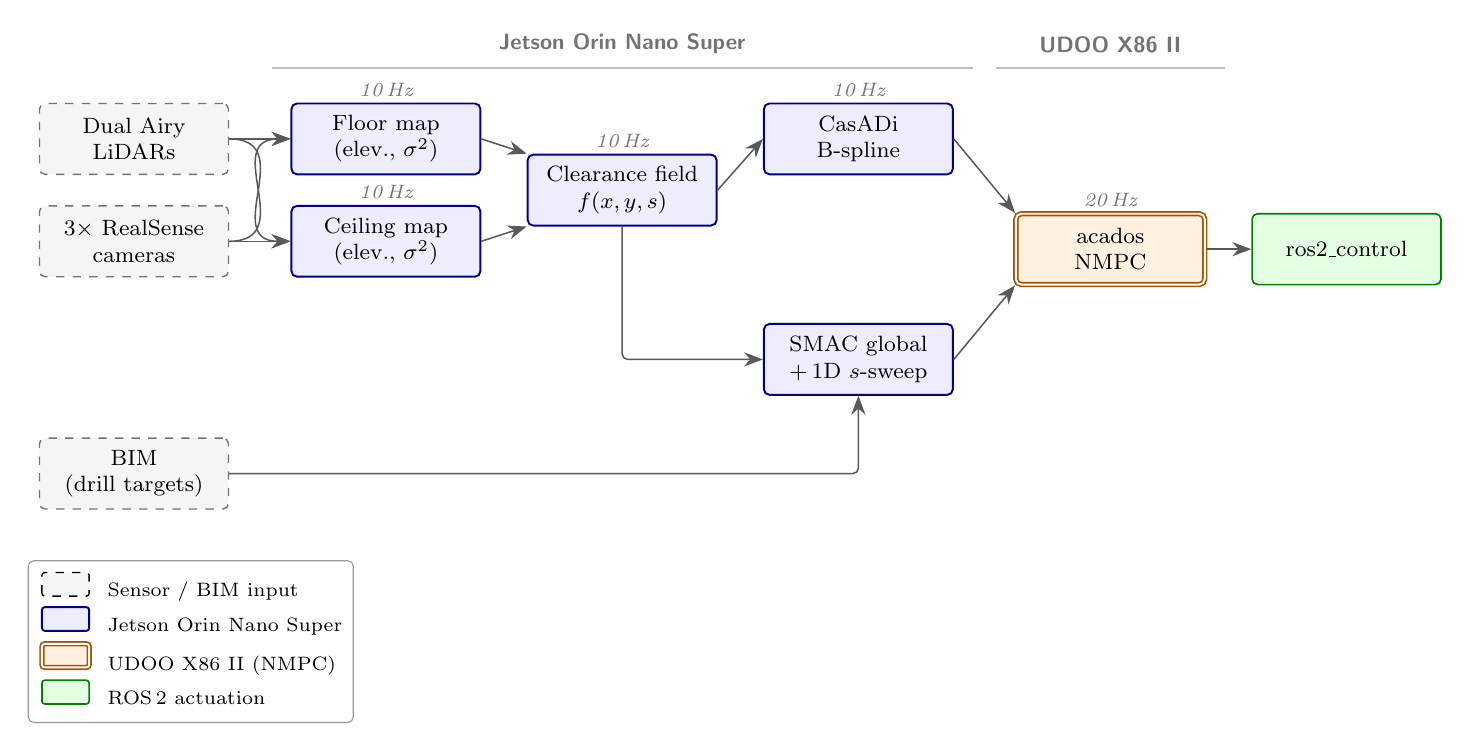
\begin{tikzpicture}[
    font=\footnotesize,
    >={Stealth[length=2.4mm,width=1.8mm]},
    every node/.style={align=center, inner sep=2.5pt},
    sensor/.style={draw=black!55, dashed, rounded corners=2pt,
                   minimum width=24mm, minimum height=9mm,
                   fill=gray!8, line width=0.5pt},
    jetson/.style={draw=blue!55!black, rounded corners=2pt,
                   minimum width=24mm, minimum height=9mm,
                   fill=blue!7, line width=0.7pt},
    udoo/.style  ={draw=orange!65!black, rounded corners=2pt,
                   minimum width=24mm, minimum height=9mm,
                   fill=orange!12, line width=0.6pt,
                   double, double distance=0.7pt},
    output/.style={draw=green!50!black, rounded corners=2pt,
                   minimum width=24mm, minimum height=9mm,
                   fill=green!10, line width=0.6pt},
    arrow/.style ={->, draw=black!65, line width=0.55pt,
                   rounded corners=2pt},
    rate/.style  ={font=\scriptsize\itshape, text=black!55,
                   inner sep=1pt},
    grouplbl/.style={font=\footnotesize\bfseries\sffamily,
                     text=black!55},
  ]

  %% --- column x-positions and row y-positions ----------------------------
  \def\xS{0}        % sensors
  \def\xM{3.2}      % mapping
  \def\xF{6.2}      % clearance field
  \def\xP{9.2}      % planning (b-spline + smac)
  \def\xC{12.4}     % control (NMPC)
  \def\xO{15.4}     % output (ros2_control)

  \def\yTop{1.85}   % top row     (LiDAR / Floor)
  \def\yMid{0.55}   % middle row  (RealSense / Ceiling)
  \def\yLow{-0.95}  % lower row   (SMAC)
  \def\yBim{-2.40}  % bottom row  (BIM)

  %% --- input nodes -------------------------------------------------------
  \node[sensor] (lidar) at (\xS,\yTop) {Dual Airy\\LiDARs};
  \node[sensor] (rs)    at (\xS,\yMid) {$3\times$ RealSense\\cameras};
  \node[sensor] (bim)   at (\xS,\yBim) {BIM\\(drill targets)};

  %% --- mapping (Jetson) --------------------------------------------------
  \node[jetson] (floor) at (\xM,\yTop) {Floor map\\(elev., $\sigma^2$)};
  \node[jetson] (ceil)  at (\xM,\yMid) {Ceiling map\\(elev., $\sigma^2$)};

  %% --- clearance field (Jetson) ------------------------------------------
  \node[jetson] (field) at (\xF, {(\yTop+\yMid)/2}) {Clearance field\\$f(x,y,s)$};

  %% --- planning (Jetson) -------------------------------------------------
  \node[jetson] (spline) at (\xP,\yTop) {CasADi\\B-spline};
  \node[jetson] (smac)   at (\xP,\yLow) {SMAC global\\$+\,1\mathrm{D}\ s$-sweep};

  %% --- control (UDOO) ----------------------------------------------------
  \node[udoo] (nmpc) at (\xC, {(\yTop+\yLow)/2}) {acados\\NMPC};

  %% --- actuation ---------------------------------------------------------
  \node[output] (out) at (\xO, {(\yTop+\yLow)/2}) {ros2\_control};

  %% --- rate annotations --------------------------------------------------
  \node[rate, above=1pt of floor.north]  {10\,Hz};
  \node[rate, above=1pt of ceil.north]   {10\,Hz};
  \node[rate, above=1pt of field.north]  {10\,Hz};
  \node[rate, above=1pt of spline.north] {10\,Hz};
  \node[rate, above=1pt of nmpc.north]   {20\,Hz};

  %% --- compute-target group labels (above each compute zone) -------------
  \node[grouplbl] at ({(\xM+\xP)/2}, 3.05) {Jetson Orin Nano Super};
  \node[grouplbl] at (\xC, 3.05) {UDOO X86 II};
  \draw[draw=black!25, line width=0.4pt]
        ({\xM-1.45},2.75) -- ({\xP+1.45},2.75);
  \draw[draw=black!25, line width=0.4pt]
        ({\xC-1.45},2.75) -- ({\xC+1.45},2.75);

  %% --- arrows ------------------------------------------------------------
  % sensors -> mapping (parallel, plus the cross-feeds shown as gentle curves)
  \draw[arrow] (lidar.east) -- (floor.west);
  \draw[arrow] (rs.east)    -- (ceil.west);
  \draw[arrow] (lidar.east) .. controls +(0.9,0) and +(-0.9,0) .. (ceil.west);
  \draw[arrow] (rs.east)    .. controls +(0.9,0) and +(-0.9,0) .. (floor.west);

  % maps -> clearance field
  \draw[arrow] (floor.east) -- (field.north west);
  \draw[arrow] (ceil.east)  -- (field.south west);

  % field -> b-spline (top branch)
  \draw[arrow] (field.east) -- (spline.west);

  % field -> SMAC (drops down then right)
  \draw[arrow] (field.south) |- (smac.west);

  % BIM -> SMAC (bottom route, then up)
  \draw[arrow] (bim.east) -| (smac.south);

  % planning -> NMPC
  \draw[arrow] (spline.east) -- (nmpc.north west);
  \draw[arrow] (smac.east)   -- (nmpc.south west);

  % NMPC -> ros2_control
  \draw[arrow] (nmpc.east) -- (out.west);

  %% --- legend (bottom-left, compact) -------------------------------------
  \node[draw=black!40, rounded corners=2pt, anchor=north west,
        inner sep=4pt, fill=white, font=\scriptsize]
        at ({\xS-1.35},\yBim-1.10) {%
    \begin{tabular}{@{}c@{\hspace{2mm}}l@{}}
      \tikz\draw[dashed, fill=gray!8, line width=0.5pt, rounded corners=1pt]
            (0,0) rectangle (6mm,3mm); & Sensor / BIM input \\[1pt]
      \tikz\draw[draw=blue!55!black, fill=blue!7, line width=0.7pt, rounded corners=1pt]
            (0,0) rectangle (6mm,3mm); & Jetson Orin Nano Super \\[1pt]
      \tikz\draw[draw=orange!65!black, fill=orange!12, line width=0.6pt,
                 double, double distance=0.7pt, rounded corners=1pt]
            (0,0) rectangle (6mm,3mm); & UDOO X86 II (NMPC) \\[1pt]
      \tikz\draw[draw=green!50!black, fill=green!10, line width=0.6pt,
                 rounded corners=1pt]
            (0,0) rectangle (6mm,3mm); & ROS\,2 actuation \\
    \end{tabular}};

\end{tikzpicture}
}
  \caption{Proposed perception-to-control pipeline with update rates and compute allocation.}
  \label{fig:pipeline}
\end{figure}

\subsection{Dual-layer elevation mapping}
\label{sec:meth:mapping}

The environment representation builds on the GPU-accelerated \texttt{elevation\_mapping\_cupy} framework~\cite{mikiElevationMappingLocomotion2022}, extended to maintain two concurrent map instances: a floor map and a ceiling map. LiDAR returns from the dual Robosense Airy~96 sensors are split by a URDF-anchored height threshold; ceiling points are negated in the z-axis before insertion so that the standard maximum-height Kalman update logic captures the lowest overhead surface, with the sign restored on readout. Variance propagation is unaffected because $\operatorname{Var}(-z) = \operatorname{Var}(z)$, so both instances expose per-cell elevation estimates and independent Kalman-filter variances $\sigma^2_{z_\mathrm{floor}}(x, y)$ and $\sigma^2_{z_\mathrm{ceil}}(x, y)$ that are consumed by the variance-aware constraint formulation of \Cref{sec:meth:constraint}.

\subsection{Variance-aware clearance field}
\label{sec:meth:constraint}

A standalone ROS\,2 node fuses the two \texttt{GridMap} instances and computes the clearance field
\begin{equation}
\label{eq:clearance}
c(x, y) = z_\mathrm{ceil}(x, y) - z_\mathrm{floor}(x, y),
\end{equation}
and the feasibility field for a given platform configuration,
\begin{equation}
\label{eq:feasibility}
f(x, y, s) = c(x, y) - h_\mathrm{base} - s - \varepsilon(x, y),
\end{equation}
where $s$ is the combined sledge extension and $\varepsilon(x, y)$ is a spatially varying, variance-aware safety margin
\begin{equation}
\label{eq:eps_probabilistic}
\varepsilon(x, y) = \varepsilon_\mathrm{base} + \delta_\mathrm{cal} + \lambda \sqrt{\sigma^2_{z_\mathrm{ceil}}(x, y) + \sigma^2_{z_\mathrm{floor}}(x, y)},
\end{equation}
in which $\varepsilon_\mathrm{base}$ accounts for irreducible factors (drill assembly extent, platform vibration amplitude, control tracking error), $\delta_\mathrm{cal}$ is a calibration term that absorbs the documented under-reporting of Kalman variance on texture-poor and oblique surfaces, and $\lambda$ sets the confidence level. With $\lambda = 3$ the formulation corresponds to a chance constraint at the \SI{99.7}{\percent} level under the Gaussian approximation that the per-cell Kalman update implicitly enforces, structurally identical to additive constraint-tightening schemes in stochastic MPC~\cite{hewingLearningBasedModelPredictive2020,lorenzenConstraintTighteningStabilityStochastic2016} but applied at the perception layer. The field is exposed to the controller via a $C^1$-smooth CasADi B-spline interpolant updated at the elevation map rate.

\subsection{Perceptive NMPC over the augmented state}
\label{sec:meth:nmpc}

The controller solves at each cycle an OCP over augmented state $\mathbf{x} = (x, y, \theta, v, \omega, s)$ and control $\mathbf{u} = (a, \alpha, u_s)$, with unicycle kinematics augmented by empirically calibrated ICR factors and a first-order integrator on the sledge. The variance-aware clearance constraint $f(x, y, s) \geq 0$ (\Cref{eq:feasibility}) enters as a path constraint via the CasADi B-spline interpolant of \Cref{sec:meth:constraint}, formulated as a soft constraint with $L_1$ slack penalty to preserve solver feasibility under transient perception artefacts. The cost balances time-to-goal, separately weighted input-rate penalties on drive acceleration and sledge rate (reflecting the order-of-magnitude bandwidth difference between actuators), a relaxed log-barrier on $f$, and a terminal cost on the drilling pose with $s = s_\mathrm{goal}$ when a drill target is the active goal. Global guidance is supplied by the SMAC Lattice planner~\cite{macenskiOpenSourceCostAwareKinematically2025} on the floor-traversability costmap with a ceiling-aware lethal layer keyed to the current sledge extension, post-processed by a 1D forward-backward sweep that attaches an $s$-profile to each waypoint and serves as the NMPC primal warm start. The problem is solved by acados SQP-RTI~\parencite{verschueren2022acados} at \SI{20}{\hertz}, calibrated against the empirical \SI{31}{\milli\second} median on a 12-state UAV model on the same hardware~\parencite{enrico2025nmpcmppi}. Gradient-based NMPC was chosen over the two surviving alternatives of \Cref{sec:sq4:discussion}: hierarchical MPC~\cite{bendersEmbeddedHierarchicalMPC2025} requires an offline terminal-set construction under an anisotropic disturbance set that has no published precedent for this kinematic class, and CBF-augmented MPPI~\cite{yin2023shieldmppi,parwana2025brmppi} enforces safety only on the committed control, which cannot anticipate the multi-second sledge-actuation timescale that couples clearance to configuration.

\subsection{Goal selection through approach-aware filtering}
\label{sec:meth:goals}

Goal selection consumes BIM-derived drill targets and emits ratified base poses. For each target, candidate base stances offset along the drill axis are filtered by two checks against the clearance field of \Cref{sec:meth:constraint}: (i) terminal feasibility $c(x, y) - h_\mathrm{base} - s_\mathrm{goal} - \varepsilon(x, y) \geq \delta_\mathrm{margin}$ at the candidate pose; and (ii) approach-corridor feasibility, verified by forward-simulating the controller's intended retraction-and-extension profile along a short approach corridor. Multi-target sequencing uses greedy nearest-neighbour with reconfiguration cost integrated against the same clearance field, addressing the approach-aware IRM gap (G4).

\subsection{Embedded deployment}
\label{sec:meth:embedded}

The complete pipeline executes within the Orin Nano Super's \SI{8}{\giga\byte} unified memory and \SI{50}{\milli\second} latency budget for a \SI{20}{\hertz} control rate. \Cref{tab:timing} allocates the budget across pipeline stages, with mapping and constraint-field computation running asynchronously at \SI{10}{\hertz} while the controller closes the loop against the most recent constraint data.

\begin{table}[htbp]
\centering
\caption{Target timing budget for the perception--planning pipeline on Jetson Orin Nano Super.}
\label{tab:timing}
\small
\setlength{\tabcolsep}{6pt}
\begin{tabularx}{\linewidth}{@{}l r r >{\raggedright\arraybackslash}X@{}}
\toprule
Stage & Target & Rate & Basis \\
\midrule
Dual elevation map update & \SI{20}{\milli\second} & \SI{10}{\hertz} & Two instances~\parencite{mikiElevationMappingLocomotion2022} \\
Constraint field (fused kernel) & \SI{0.1}{\milli\second} & \SI{10}{\hertz} & Profiled: $< \SI{60}{\micro\second}$ \\
Clearance to B-spline coefficients & \SI{1}{\milli\second} & \SI{10}{\hertz} & CasADi interpolant update \\
SMAC + 1D sweep warm-start & \SI{2}{\milli\second} & \SI{10}{\hertz} & SMAC + sweep~\parencite{macenskiOpenSourceCostAwareKinematically2025} \\
NMPC solve & \SIrange{5}{20}{\milli\second} & \SI{20}{\hertz} & acados~\parencite{verschueren2022acados,enrico2025nmpcmppi} \\
Safety monitor + DDS overhead & \SI{2}{\milli\second} & \SI{20}{\hertz} & Zenoh bridge, measured \\
\midrule
Total (worst case) & $\sim$\SI{45}{\milli\second} & & Margin: \SI{5}{\milli\second} \\
\bottomrule
\end{tabularx}
\end{table}

\subsection{Research plan}
\label{sec:methodology:validation}

The research plan proceeds in six phases:

\begin{enumerate}
\item \textbf{Perception backbone.} Implement the dual-instance elevation mapping of \Cref{sec:meth:mapping} with z-inversion encoding for the ceiling layer, validated against laser-measured ceiling reference points to verify that the mapping MAE is bounded relative to the irreducible margin $\varepsilon_\mathrm{base}$.

\item \textbf{Constraint field and variance calibration.} Implement the variance-aware clearance field of \Cref{sec:meth:constraint} as a fused CUDA kernel, with the calibration term $\delta_\mathrm{cal}$ fit offline against a held-out set of indoor ceiling sequences to absorb the documented under-reporting of Kalman variance on texture-poor surfaces.

\item \textbf{Controller implementation.} Implement the perceptive NMPC of \Cref{sec:meth:nmpc} in CasADi with the acados SQP-RTI backend, profiled in simulation against a fixed-$s$ baseline to confirm the joint-optimisation hypothesis.

\item \textbf{Comparative evaluation in Gazebo.} Evaluate the proposed controller against two baselines (an always-retract baseline representing the current industrial operational envelope, and a decoupled baseline pairing the global planner with a 1D height sweep) across environments stressing ceiling-height variation, perception variance perturbation, SLAM drift, and ceiling complexity. The variance-aware tightening contribution is isolated through an ablation that fixes $\delta_\mathrm{cal} = 0$, $\lambda = 0$.

\item \textbf{Embedded characterisation.} Profile the complete pipeline on the Jetson Orin Nano Super under load to confirm the latency budget of \Cref{tab:timing}, with per-component timing, peak unified-memory occupancy, and DDS communication latency across the dual-computer architecture.

\item \textbf{Hardware validation.} Reproduce the headline ceiling-clearance scenario at the industrial partner facility with adjustable-height crossbars and total-station ground truth, comparing the proposed controller against the always-retract baseline to quantify the sim-to-real gap.
\end{enumerate}

\begin{figure}[t]
  \centering
  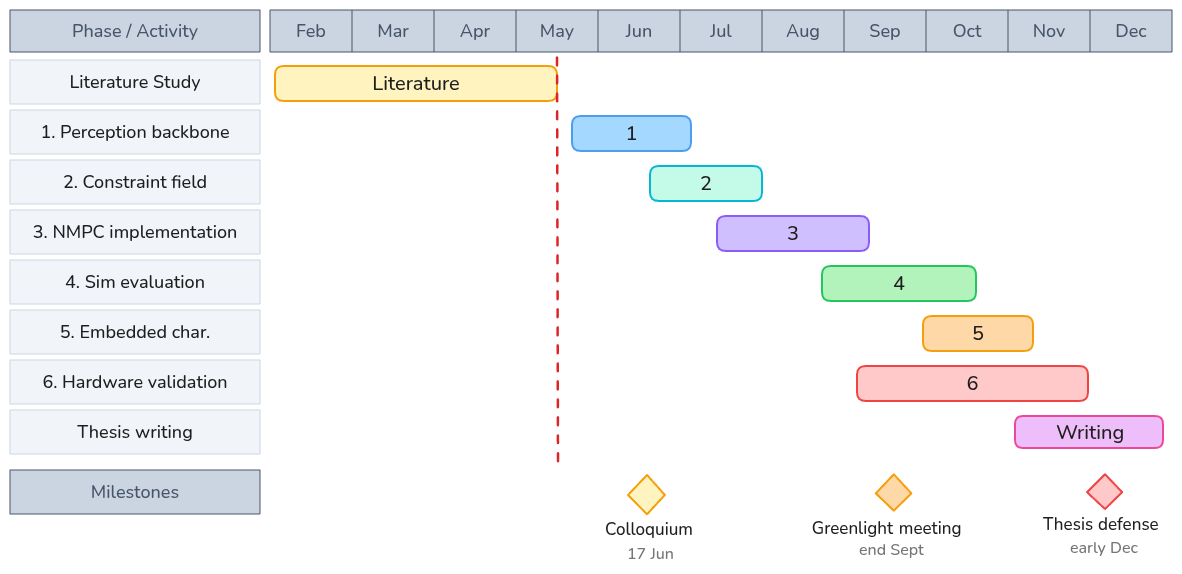
\includegraphics[width=\linewidth]{figures/images/timeline.png}
  \caption{Project timeline through colloquium and ICRA 2027 submission.}
  \label{fig:timeline}
\end{figure}

\newpage
\printbibliography

\end{document}
